\documentclass[1p]{elsarticle}

\usepackage{lineno,hyperref}
\modulolinenumbers[5]

\journal{Journal of \LaTeX\ Templates}

%%%%%%%%%%%%%%%%%%%%%%%
%% Elsevier bibliography styles
%%%%%%%%%%%%%%%%%%%%%%%
%% To change the style, put a % in front of the second line of the current style and
%% remove the % from the second line of the style you would like to use.
%%%%%%%%%%%%%%%%%%%%%%%

%% Numbered
%\bibliographystyle{model1-num-names}

%% Numbered without titles
%\bibliographystyle{model1a-num-names}

%% Harvard
%\bibliographystyle{model2-names.bst}\biboptions{authoryear}

%% Vancouver numbered
%\usepackage{numcompress}\bibliographystyle{model3-num-names}

%% Vancouver name/year
%\usepackage{numcompress}\bibliographystyle{model4-names}\biboptions{authoryear}

%% APA style
\bibliographystyle{model5-names}\biboptions{authoryear}

%% AMA style
%\usepackage{numcompress}\bibliographystyle{model6-num-names}

%% `Elsevier LaTeX' style
%\bibliographystyle{elsarticle-num}
%%%%%%%%%%%%%%%%%%%%%%%

% ---------------------
% Pacotes OBRIGATÓRIOS
% ---------------------
\usepackage{lmodern}				% Usa a fonte Latin Modern			
\usepackage[T1]{fontenc}			% Selecao de codigos de fonte.
\usepackage[utf8]{inputenc}		% Codificacao do documento (conversão automática dos acentos)
%\usepackage{lastpage}			% Usado pela Ficha catalográfica
%\usepackage{indentfirst}			% Indenta o primeiro parágrafo de cada seção.
\usepackage{color}			     	% Controle das cores
\usepackage{graphicx}	         % Inclusão de gráficos
\usepackage{epsfig,subfig}		% Inclusão de figuras
\usepackage{microtype} 			% Melhorias de justificação
% ---------------------

% ---------------------
% Pacotes ADICIONAIS
% ---------------------
\usepackage{lipsum}						% Geração de dummy text
\usepackage{amsmath,amssymb,mathrsfs, amsthm}	% Comandos matemáticos avançados 
\usepackage{setspace}  					% Para permitir espaçamento simples, 1 1/2 e duplo
\usepackage{verbatim}					% Para poder usar o ambiente "comment"
\usepackage{tabularx} 					% Para poder ter tabelas com colunas de largura auto-ajustável
\usepackage{afterpage} 					% Para executar um comando depois do fim da página corrente
\usepackage{url} 						% Para formatar URLs (endereços da Web)
\usepackage{todonotes}  				% Lista de afazeres To-dos
\usepackage{enumitem}					% Fazer enumerações por letras ou números nos itens
\usepackage{float}
\usepackage{longtable}					% Tabelas que se estendem por mais de uma página
\usepackage{booktabs}					% Tabelas com multicolunas
\usepackage[brazil]{babel}				% Pacote de tradução

% Configura o ambiente de teoremas, definições etc.

\theoremstyle{definition} 
\newtheorem{teor}{Teorema}%[section]
\newtheorem{defi}[teor]{Definição}
\newtheorem{lema}[teor]{Lema}
\newtheorem{supo}[teor]{Suposição}
\newtheorem{exemplo}[teor]{Exemplo}
\newtheorem{prop}[teor]{Proposição}


\begin{document}
	
\begin{frontmatter}

\title{Aplicando a teoria do valor extremo no cálculo de risco de índices setoriais da Bovespa\tnoteref{titlenote}}
\tnotetext[titlenote]{Agradecemos a FAPESC pelo o apoio ao desenvolvimento da pesquisa que resultou no presente artigo.}

%\title{Medidas condicionais de risco através da teoria do valor extremo}%\tnoteref{mytitlenote}}
%\tnotetext[mytitlenote]{Fully documented templates are available in the elsarticle package on \href{http://www.ctan.org/tex-archive/macros/latex/contrib/elsarticle}{CTAN}.}

%% Group authors per affiliation:
%\author{Rafael Felipe Bressan\fnref{myfootnote}\corref{correspondente}}
%\cortext[correspondente]{Autor para correspondência}
%\ead{rafael.bressan@edu.udesc.br}
%\author{Daniel Augusto de Souza\fnref{myfootnote}}
%\address{Avenida Madre Benvenuta, 2007 - Santa Mônica Florianópolis - SC 88035-901}
%\fntext[myfootnote]{Depto. de Economia/Esag/UDESC}

%% or include affiliations in footnotes:
%\author[mymainaddress,mysecondaryaddress]{Elsevier Inc}
%\ead[url]{www.elsevier.com}

\author[mymainaddress]{Rafael Felipe Bressan\corref{mycorrespondingauthor}\fnref{myfootnote}}
\cortext[mycorrespondingauthor]{Autor para correspondência}
\ead{rfbressan@gmail.com}
\fntext[myfootnote]{Depto. de Economia/Esag/UDESC}
%
\author[mymainaddress]{Daniel Augusto de Souza\fnref{myfootnote}}
\author[mymainaddress]{Adriano de Amarante\fnref{myfootnote}}

\address[mymainaddress]{Avenida Madre Benvenuta, 2007 - Santa Mônica Florianópolis - SC 88035-901}
%\address[mysecondaryaddress]{360 Park Avenue South, New York}

\listoftodos

\begin{abstract}
	Este trabalho faz um comparativo entre dois modelos univariados de estimação de valor em risco para seis índices de ações calculados na Bovespa. Os modelos testados são do tipo condicional e um período fora da amostra com mais de 3 anos de observações diárias é utilizado. A partir de dois procedimentos de avaliação, cobertura incondicional e teste de independência de violações, os melhores resultados são apresentados pelo modelo que une a teoria do valor extremo e modelagem condicional de variâncias heterocedásticas, o qual leva em conta o regime variável nas volatilidades das perdas assim como excesso de curtose. Em seguida uma comparação entre os níveis médios de risco entre os índices é analisado com o intuito de auferir quais índices se mostram os mais arriscados para o investidor.
\end{abstract}

\begin{keyword}
Value-at-Risk \sep Extreme Value Theory \sep Peaks over Threshold \sep Conditional EVT \sep GARCH models
\end{keyword}

\end{frontmatter}

\linenumbers

\section{Introdução}

Pode-se definir risco como o grau de incerteza dos retornos líquidos futuros. Essa incerteza assume muitas formas, razão pela qual a maioria dos participantes nos mercados financeiros está sujeita a uma variedade de riscos. Uma classificação comum dos riscos baseia-se na fonte da incerteza subjacente.

No setor financeiro, o tipo de risco mais conhecido é provavelmente o \emph{risco de mercado}, o risco de mudança no valor de uma posição financeira devido a mudanças no valor do subjacente dos componentes em que essa posição depende, tais como preços de ações e títulos, taxas de câmbio, preços de commodities, etc.

A medição do risco de mercado ao qual os portfólios dos investidores está sujeito é objeto de devoção de esforços tanto por parte das instituições e investidores em geral como por parte dos reguladores. Instituições financeiras - IF em todo o mundo, de acordo com suas regulações locais e com os princípios de Basileia (\emph{Basel Comittee on Banking Supervision} - BCBS do Banco de Compensações Internacionais - BIS) são obrigadas a reservar uma parcela de seu capital como provisionamento contra flutuações adversas do mercado, como forma de mitigar seu risco de insolvência.

%Estas instituições devem manter seu risco de insolvência controlado, e a percepção externa deve ser tal que não haja desconfiança do público com sua habilidade em controlar este risco. Se a confiança na instituição se esvai e a percepção de risco é elevada, rapidamente uma crise de liquidez pode surgir, com depositantes sacando seus recursos ao mesmo tempo em que outras fontes de \emph{funding} também se tornam escassas. %Em tal situação, é natural o banco ou IF, ir ao mercado para vender seus ativos e levantar os recursos necessários. Neste momento uma crise de liquidez no mercado pode levar a uma possível insolvência da IF pois, não há garantias que no mercado aberto, os ativos do banco serão justamente avaliados e arrematados.

Uma importante característica das séries de retornos financeiros é sua alta volatilidade, não constante e tampouco seguindo uma distribuição Normal. Assim, eventos extremos, e neste caso estamos interessados em perdas de grande magnitude, acontecem com uma frequência alta demais para serem descartadas como apenas \emph{outliers}, e portanto passaram a atrair a atenção dos participantes do mercado, entre eles os investidores e reguladores. Estas observações induziram uma gama de estudos, empíricos e teóricos, voltados a explicar o comportamento dos retornos de séries financeiras e modelar de forma adequada as caudas da distribuição destes retornos. Não somente estes estudos são de grande relevância para o gerenciamento de risco nas instituições financeiras, como também são obrigatórios segundo o acordo de Basileia, uma vez que este requer o cálculo do Valor em Risco - VaR, para então a instituição poder projetar o seu nível requerido de capital. 

%De acordo com os princípios de Basileia III, \cite{BankingSupervision2011, BankingSupervision2013, BankingSupervision2014}, as instituições financeiras supervisionadas pelos Bancos Centrais devem manter \emph{buffers} de capital contra riscos de mercado, crédito, liquidez, entre outros. 
Dentro dos riscos de mercado, as duas formas mais usuais de fazer a quantificação destes são os métodos de Valor em Risco - VaR e o \emph{Expected Shortfall} - ES. Este último relacionado ao primeiro, sendo definido como o valor esperado das perdas que excedem o VaR calculado para um determinado nível de confiança e horizonte temporal. VaR é um quantil alto $\alpha$ da distribuição de perdas de um ativo ou portfólio em um determinado período de tempo, ao passo que ES é o valor esperado das perdas que excedem VaR, para um mesmo período e nível de confiança $\alpha$.

O método VaR para cálculo de risco de mercado ao qual um portfólio está sujeito foi primeiramente introduzido através de \cite{RiskMetrics1995}, uma metodologia adotada pelo banco J. P. Morgan. Vem desde então sendo amplamente adotado pela indústria financeira e largamente estudado pela academia. Inúmeras variantes do modelo foram propostas e continuam sendo utilizadas com o passar dos anos. Para o cálculo do VaR é necessária uma suposição acerca da distribuição dos retornos, e por conseguinte do comportamento da cauda desta.

%As variações na metodologia original de estimação do VaR surgem principalmente em função de críticas a abordagem proposta, a qual inclui a suposição de retornos independentes e igualmente distribuídos, covariâncias constantes entre os ativos de um portfólio e a distribuição normal dos retornos. 

%Por meio de dois artigos \cite{Artzner1997} e \cite{Artzner1999}, foi introduzido na literatura o conceito de medida coerente de risco. Para uma medida ser considerada coerente, primeiramente foram introduzidas quatro propriedades cunhadas através de axiomas, as quais estas medidas deveriam possuir, invariância translacional, sub-aditividade, homogeneidade positiva, e monotonicidade.
%
%VaR especificamente não possui a propriedade da sub-aditividade para alguns casos, sendo esta uma das grandes críticas ao VaR. Desta forma, em casos específicos, é possível uma carteira diversificada em que sejam computados o VaR de cada um de seus ativos, ser agregada e possuir um VaR do portfólio maior que o maior VaR de seus componentes, algo que não condiz com uma medida coerente de risco. Para contornar este fato, \cite{Acerbi2002} propuseram o \emph{Expected Shortfall} e comprovam que este é uma medida coerente de risco. Além de ser coerente, o ES possui uma segunda vantagem com relação ao VaR, considerando que o ES nos informa uma medida de tendência central do tamanho das perdas que excedem o valor do quantil VaR. Ou seja, o VaR nos informa apenas que uma proporção $\alpha$ das perdas serão menores que a medida, mas nada nos informa se esta perda extraordinária de fato ocorrer. Mesmo sendo criticado como uma medida não coerente de risco, o VaR continua a ser amplamente utilizado, mesmo que agora em conjunto com o ES. 

%Mais recentemente o Comitê de Supervisão Bancária de Basileia tem se proposto a adotar o \emph{Expected Shortfall} como medida de risco de mercado. \cite{BankingSupervision2013a}. O Comitê cita a grande importância da escolha da medida de risco e sua calibração, e portanto estas são relevantes para as decisões de política do Banco. Entre as dificuldades encontradas pelo VaR estão mais notadamente sua inabilidade em estimar o "risco de cauda" da distribuição de perdas, uma vez que VaR não leva em conta a distribuição das perdas acima do valor de corte.

%Desta forma, foi decidido que o ES seria a medida de risco favorita para a abordagem pelo banco chamada de modelos internos. Ou seja, os bancos supervisionados devem utilizar o ES para o cálculo do risco de mercado a que estão sujeitos em seus modelos internos. O comitê também se decidiu por um nível de confiança de 97,5\% para o ES, em contraposição a 99\% para o VaR. O comitê espera que esta abordagem para o cálculo da medida de risco de mercado trará benefícios se comparada a antiga abordagem pelo Var, entre elas um modelo com resultados mais estáveis e menor sensibilidade a observações extremas (\emph{outliers}).

Teoria do valor extremo - EVT, é um ramo da estatística que lida diretamente com eventos raros, extremos. Seu objetivo é modelar o comportamento assintótico de eventos que se distanciam muito da mediana de uma distribuição. Justamente por esta característica, a EVT está sendo utilizada para modelar riscos que possuem distribuição com caudas longas, um dos fatos estilizados bem conhecidos sobre retornos de ativos financeiros.

Ao utilizar a EVT, e mais especificamente o método conhecido como \emph{peaks over treshold} – POT, se está interessado em modelar apenas a parte da cauda da distribuição das perdas de um ativo financeiro maiores que um determinado valor de limiar \emph{u}. É da modelagem desta cauda, portanto, que se calcula a estimativa de VaR.

A teoria do valor extremo vem sendo utilizada nas finanças a algum tempo. Devido as características das séries financeiras, por exemplo a leptocurtose, a distribuição normal para os retornos vem sendo rechaçada, enquanto outras distribuições mais adequadas assumem o posto para descrever o comportamento das perdas e retornos de séries financeiras. A EVT, ao modelar distribuições com caudas longas, pode ser utilizada para esta finalidade. A introdução da EVT em dois estágios para a estimação de medidas condicionais de risco pode ser atribuída a \cite{McNeil2000}. Naquele artigo os autores propuseram um modelo para a estimação do VaR e ES de forma condicional, tanto para período de um dia como para dez dias a frente, de acordo com o normativo de Basileia vigente a época. Seu modelo, que leva em conta as longas caudas e a natureza estocástica da volatilidade, se ajustam de forma mais fidedigna aos dados. \cite{Danielsson2000} fizeram uma crítica aos modelos condicionais de cálculo do VaR para o mercado japonês e chegaram a conclusão que um modelo EVT incondicional, inclusive sem o estágio de filtragem inicial, era mais adequado para fins práticos.

\cite{Bystroem2004} encontrou que ambas abordagens da EVT, máximos em bloco como POT, combinadas com análise de séries temporais tradicional (ARIMA e GARCH), no que se configura uma abordagem condicional para a estimação do VaR, têm os melhores resultados tanto em períodos ditos tranquilos como em épocas de alta volatilidade. Voltando a aplicação da EVT para mercados emergentes, \cite{Gencay2004} utilizaram a teoria de valor extremo para o cálculo de VaR e teste de estresse. Seus resultados apontam que a EVT se torna melhor a medida que o quantil utilizado para o cálculo se eleva. Além disso, encontraram que as caudas da distribuição de retornos se comportam de maneira diferente entre ganhos e perdas. Uma comparação entre diversos modelos de previsão de VaR foi realizada por \cite{Kuester2006}. Encontraram que a grande maioria dos modelos subestima o risco, mesmo sendo aceitáveis do ponto de vista regulatório, sendo que o modelo condicional GARCH-EVT está entre as melhores estimações.


%\cite{Karmakar2014} retomam o modelo em dois estágios e fizeram uma comparação entre o modelo EVT condicional e outros modelos já consagrados no cálculo de VaR em 3 mercados desenvolvidos (EUA, Reino Unido e Japão) e 3 mercados emergentes asiáticos (Índia, Hong Kong e Corea do Sul). O modelo GARCH adotado no primeiro estágio é diferente para cada mercado, porém com uma particularidade comum, todos são modelos assimétricos. Novamente encontram que o modelo EVT condicional é superior aos demais através de testes de cobertura incondicional e condicional.

%\cite{Chavez-Demoulin2005} e \cite{Herrera2013} tomam um caminho diferente para modelar a EVT. Enquanto o primeiro adota o método de processos pontuais de auto-excitação\footnote{Para maiores detalhes sobre processos pontuais de auto-excitação, \cite{Hawkes1971} é a referência original.}, que dadas algumas condições, converge para o método POT, o segundo modela explicitamente as durações de tempo entre as observações de extremos, ou seja, as perdas em excesso ao limiar escolhido. A magnitude destas perdas continua a ser modelada através da distribuição generalizada de Pareto - GPD. Seu modelo é então chamado de \emph{autoregressive conditional duration peaks over threshold model} - ACD-POT.

\cite{Rocco2014} fez uma grande revisão sobre o uso da EVT em finanças. As principais aplicações encontradas  foram o teste de suposições para diferentes distribuições dos dados, cálculo de medidas de risco como o VaR e ES, alocação de ativos sob restrições e otimização de portfólios, e no estudo de contágio e dependência entre mercados sob condições de alto estresse, como em \cite{Amarante2017}.

%Mais recentemente a EVT encontrou outras formas de aplicação e cálculo. \cite{Chavez-Demoulin2016} sugeriram um modelo onde a frequência e a severidade das perdas podem ser modeladas através da EVT com covariantes.  \cite{Karmakar2016} por sua vez, fizeram uma aplicação do modelo EVT condicional a retornos intra-diários de dezesseis mercados diferentes.

O cálculo de VaR em instituições financeiras e bancos comerciais vem sendo implementado e é requerimento do comitê de Basileia. A EVT entra como uma das metodologias utilizadas neste cálculo,  \cite{Longin2000} a utilizou e propôs um modelo para agregar o risco de uma posição de mercado, em contraste a modelos univariados apenas. Testes de estresse podem ser realizados através de sua técnica. Utilizando-se de dados reais de seis grandes bancos comerciais americanos, \cite{Berkowitz2002} analisou a precisão de seus modelos VaR. Ele encontrou que os bancos são amplamente conservadores em suas estimativas de VaR, com níveis de cobertura muito acima dos valores nominais. \cite{Wong2003} promoveu um estudo sobre as implicações da precisão do modelo VaR no gerenciamento do risco de mercado em bancos. Ele adotou os critérios de Basileia para realizar um estudo de \emph{backtest} e verificou que modelos baseados em previsões de volatilidade através de GARCH não estão de acordo com estes critérios por muitas vezes. Já em um estudo recente, \cite{OBrien2017} fez uma avaliação dos modelos de risco de mercado de bancos no pré, durante e pós crise financeira de 2008. Encontrou que tanto no pré quanto no pós crise, os bancos se comportaram de maneira excessivamente conservadora, entretanto, durante a crise financeira as violações ao VaR excederam muito seu valor esperado assim como aconteceram de forma agrupada, um sinal de má especificação nos modelos adotados. O autor comparou estes resultados com um modelo baseado em GARCH e verificou que esta alternativa é muito superior aos atuais modelos.

Este artigo busca avaliar, através de testes estatísticos, a capacidade preditiva de dois modelos distintos de cálculo da métrica de valor em risco comumente encontrados na literatura, por meio da técnica de \emph{backtest}. O modelo EVT condicional em dois estágios, proposto por \cite{McNeil2000}, e o modelo associados ao grupo \emph{RiskMetrics}, que pressupõe distribuição normal dos retornos. Os testes aplicados abrangem características importantes do VaR como cobertura incondicional e independência entre violações.

O restante deste artigo está assim organizado, na seção \ref{sec:caudas} é apresentada a teoria do valor extremo, seus principais resultados para séries \emph{iid} utilizando o método \emph{peaks over treshold} e o modelo em dois estágios com filtragem inicial a partir de um modelo AR-GARCH. Na seção \ref{sec:descritivas} são apresentados os índices e seus períodos em análise. Algumas estatísticas descritivas dos retornos são calculadas. Já em \ref{sec:filtro} e \ref{sec:metpot} o modelo EVT condicional utilizado é revisto e seus parâmetros de análise são determinados a partir de uma amostra de trabalho (período dentro da amostra). Em \ref{sec:avaliacao}, a avaliação no período fora da amostra dos modelos é realizada, testes estatísticos para cobertura condicional e incondicional são feitos na subseção \ref{sec:testes}. Um comparativo entre os níveis de risco de cada um dos índices analisados é apresentado em \todo{Seção comparando níveis de risco. \ref{label}}. Ao final, uma conclusão sobre os resultados encontrados e no \ref{apendice} são apresentados em maiores detalhes os modelos analisados.

\section{Modelando caudas e medidas de risco associadas com EVT}
\label{sec:caudas}

Considere uma amostra de uma variável aleatória - \emph{va} - cujas observações sejam independentes e igualmente distribuídas - \emph{iid}, $X_i$, com $i\in \mathbb{N}$, que representem as perdas financeiras de um determinado ativo, com uma função de distribuição - \emph{df} - desconhecida $F(x) = P(X_i \leq x)$.
Seja \emph{u} um valor de limiar a partir do qual perdas acima deste valor sejam consideradas extremas. Os valores de excesso serão, portanto, $X_i - \emph{u}$.

A EVT está interessada em investigar o comportamento da distribuição dos máximos desta \emph{va} dados por $M_n = \max (X_1, \ldots , X_n)$ para valores de $n$ a medida que $n\rightarrow \infty$. A sequência $M_n$ é chamada de máximos em bloco e foi demonstrado através do conhecido teorema de Fisher-Tippett-Gnedenko\footnote{Os três artigos que fundamentam este teorema são: \cite{Fisher1928}, \cite{Gnedenko1941, Gnedenko1943}.}, que a única distribuição para a qual $M_n$ converge com $n\rightarrow \infty$ é a distribuição de valores extremos generalizada - GEV. Se esta distribuição for denotada por $H_\xi$, com $\xi$ um parâmetro da distribuição, então se diz que $F \in MDA(H_\xi)$, $F$ pertence ao domínio de máxima atração de $H_\xi$.

\begin{defi}[GEV] \label{defi:GEV}
	Distribuição de valores extremos generalizada, é definida por sua função densidade de probabilidade - pdf - a qual é dada por:
	
	\begin{equation}
	\label{eq:GEV}
	H_\xi(x) = 
	\begin{cases}
	exp(-(1+\xi x)^{-\frac{1}{\xi}}), & \xi \neq 0,\\
	exp(-e^{-x}), & \xi = 0,\\
	\end{cases}
	\end{equation}
\end{defi}

O parâmetro $\xi$ é conhecido como parâmetro de forma da distribuição e dependendo deste valor tem-se diferentes tipos de distribuição (casos particulares da GEV). %Quando $\xi=0$ a distribuição resultante é uma Gumbel, quando  $\xi>0$ uma Fréchet surge, e por fim quando $\xi<0$ tem-se uma Weibull.

Para as aplicações financeiras não necessitamos calcular a qual $MDA$ pertencem nossas distribuições contínuas, bastando saber que basicamente todas as distribuições de utilidade prática estão contidas em $MDA(H_\xi)$ para algum valor de $\xi$ \cite[p. ~139]{McNeil2015}.

\subsection{Excessos acima de um limiar}
\label{sec:excess}

O método POT para calcular a função de distribuição dos valores que excedem um determinado limiar de um conjunto de dados vem sendo empregado no mundo financeiro para ajustar as caudas das distribuições de retornos, ou perdas, dos ativos. Este método é preferido aquele de máximos em bloco, pois, desperdiça uma quantidade menor de dados da série original. Qualquer valor que exceda o limiar pré-determinado é considerado na distribuição dos excessos. Esta, por sua vez, é definida como:

\begin{defi}[Distribuição dos excessos] \label{defi:excess}
	Seja \emph{X} uma variável aleatória com função de distribuição \emph{F}. A distribuição dos excessos sobre um limiar \emph{u} tem a seguinte função de distribuição:
	
	\begin{equation}
	\label{eq:excessdist}
	F_u(x)=P(X-u \leq x | X > u)=\frac{F(x+u)-F(u)}{1-F(u)}
	\end{equation}
	para $0 \leq x < x_F-u$, onde $x_F \leq \infty$ é o limite direito da distribuição \emph{F}.
\end{defi}

Uma importante distribuição que surge na modelagem dos excessos sobre um limiar é a distribuição gereralizada de Pareto – GPD, que segue.

\begin{defi}[GPD] \label{defi:GPD}
	A função de distribuição de Pareto Generalizada é definida como:
	\begin{equation}
	\label{eq:GPD}
	G_{\xi,\psi}(x) = 
	\begin{cases}
	1- \left(1+ \frac{\xi x}{\psi} \right)^{-\frac{1}{\xi}}, & \xi \neq 0,\\
	1-exp\left(-\frac{x}{\psi}\right), & \xi = 0,\\
	\end{cases}
	\end{equation}
	onde $\psi > 0$, e $x\geq 0$ quando $\xi  \geq 0$ ou $0 \leq x \leq -\psi / \xi$ quando $\xi < 0$.
\end{defi}

Os parâmetros $\xi$ e $\psi$ são conhecidos respectivamente como parâmetros de forma e escala da distribuição. A GPD tem papel fundamental na teoria de valor extremo em função do teorema de Pickands-Balkema-de Haan\footnote{As referências originais são: \cite{Pickands1975} e \cite{Balkema1974}.}, onde é demonstrado que, para um valor suficientemente alto do limiar \emph{u}, a distribuição dos excessos $F_u(x)$ pode ser aproximada por uma GPD, $G_{\xi,\psi}(x)$.

O que este teorema prova é que para distribuições as quais os máximos em bloco normalizados convergem para uma GEV na forma da equação \eqref{eq:GEV}, então a distribuição dos excessos acima de um limiar destas mesmas distribuições convergem para \eqref{eq:GPD}, dado um valor de limiar \emph{u} adequado. Como para fins práticos basicamente todas as distribuições contínuas de fato estão no $MDA(H_\xi)$ para algum valor de $\xi$, temos que a GPD é a distribuição a ser escolhida para modelar excessos acima de um limiar.

Ao se fazer esta suposição que a distribuição dos excessos \emph{é igual} a \eqref{eq:GPD}, pode-se então, a partir dos dados, estimar os parâmetros de forma e escala e, portanto, modelar a cauda direita da distribuição de perdas de forma parametrizada com o auxílio da equação \eqref{eq:excessdist}. 


Dada a parametrização de uma GPD, é interessante saber o valor esperado desta distribuição, uma vez que esta medida de valor central fornece importante informação sobre a quantidade de risco que se está medindo, assim como a informação de que a própria distribuição foi ajustada aos dados de forma satisfatória.

O valor esperado de uma variável aleatória não negativa pode ser computado através da integral de sua cauda, $P(X>x) = 1-P(X \leq x)$. A cauda de \eqref{eq:GPD} é, para $\xi \neq 0$, $\left(1+\xi x / \psi \right)^{-1/ \xi}$.

Desta forma, o valor esperado de $G_{\xi,\psi}(x)$, converge para:

\begin{equation}
\label{eq:meanGPD}
E\left[G_{\xi,\psi} (X) \right]=\frac{\psi}{1-\xi}
\end{equation}
desde que $\xi<1$.

\begin{defi}[função média dos excessos]
	\label{defi:meanexcess}
	A função média dos excessos de uma variável aleatória \emph{X} com média finita é dada por:

	\begin{equation}
	\label{eq:meanexcess}
	e(u)=E\left(X-u | X > u\right)
	\end{equation}
\end{defi}

Ou seja, a equação \eqref{eq:meanexcess} representa o valor esperado da função de distribuição dos excessos dada pela Definição \ref{defi:excess}. Ela representa a média de $F_u$ como uma função do limiar \emph{u}. Por vezes também é conhecida como função média de vida residual (\emph{mean residual life function}).

Para uma variável distribuída na forma de $G_{\xi,\psi}(x)$, o parâmetro de escala é uma função linear em \emph{u} dado por $\psi(u)=\psi + \xi u$, \cite[Teorema 3.4.13(e)]{Embrechts1997}. Utilizando-se deste fato e da equação \eqref{eq:meanGPD} chegamos ao cálculo da função média dos excessos para uma GPD, dada por:

\begin{equation}
\label{eq:eu}
e(u)=\frac{\psi+\xi u}{1-\xi}
\end{equation}
onde $0 \leq u < \infty$ se $0 \leq \xi <1$ e $0 \leq u \leq -\psi / \xi$ se $\xi < 0$. É possível observar que de fato a função média dos excessos é linear em \emph{u}. Esta é uma característica importante de uma distribuição de Pareto generalizada e que pode ser utilizada para auxiliar a escolha de um valor adequado do limiar \emph{u} de tal forma que a suposição de convergência $F_u(x) \rightarrow G_{\xi, \psi}(x)$ seja válida.

Assim, quando da análise de uma determinada distribuição de perdas \emph{F} e se deseja ajustar a cauda desta para perdas acima de um valor limiar \emph{u} a uma GPD, é necessário primeiramente determinar um valor adequado de \emph{u} que garanta a suposição de convergência. Um método frequentemente utilizado é o gráfico da função média dos excessos com relação a \emph{u}. Analisando este gráfico, escolhe-se o menor valor de \emph{u} para o qual a partir deste ponto a relação $e(u) \text{ vs } u$ torna-se linear.

Deseja-se o menor valor de \emph{u} para o qual a relação é linear pois, mesmo o método POT implica em grande perda de observações da série temporal, já que apenas os valores acima deste limiar são utilizados para fazer a estimação dos parâmetros $\xi$ e $\psi$ da GPD. Portanto, existe um \emph{trade-off} na escolha do valor limiar \emph{u}, escolhendo um valor muito baixo obtém-se uma boa quantidade de dados para estimar os parâmetros da GPD, mas a própria distribuição resultante não será GPD, uma vez que não estaremos trabalhando na região onde a relação $e(u) \text{ vs } u$ é linear, e portanto os parâmetros estimados serão viesados. Por outro lado, um valor limiar muito alto impõe o custo de trabalhar com poucos dados para fazer a estimação dos parâmetros da distribuição e por conseguinte, os erros padrões dessas estimativas serão elevados.

Considerando este \emph{trade-off}, uma saída é buscar minimizar o erro quadrado médio - MSE do parâmetro estimado. Idealmente deseja-se ter viés zero e variância mínima para um estimador entretanto, na impossibilidade de tal realização, um estimador relativamente eficiente é aquele que possui o menor MSE. Em \cite[seção 5.2.5, p. ~161-162]{McNeil2015} é explorada, através de simulação de Monte Carlo, esta relação entre a escolha do limiar \emph{u} e o MSE do parâmetro $\xi$ obtido através do método POT e também da própria medida de risco $VaR_{99\%}$. Chegam a conclusão que uma escolha de limiar tal que o número de excessos a este fique acima de 100 observações é adequado, e mais importante, a partir destas 100 observações o MSE é relativamente robusto, se elevando lentamente a partir de seu valor mínimo.

\subsection{Estimando o VaR}
\label{sec:var}

Através da modelagem da cauda da distribuição \emph{F} de perdas por uma GPD, é possível calcular de forma semi-paramétrica a medida de risco VaR em função dos parâmetros estimados de \eqref{eq:GPD} e da distribuição empírica de \emph{F}.

Sob a suposição de convergência a cauda da distribuição \emph{F}, $\bar{F}(x)$, para $x \geq u$ é dada por:

\begin{align}
\label{eq:Ftail}
\bar{F}(x) & = P(X>u)P(X>x|X>u) \nonumber \\
& = \bar{F}(u) P(X-u>x-u|X>u) \nonumber \\
& = \bar{F}(u)\bar{F}_u(x-u) \nonumber \\
& = \bar{F}(u)\left(1+\xi \frac{x-u}{\psi}\right)^{-1/\xi}
\end{align}

Aqui $x$ são os valores a serem observados das perdas, e portanto $x-u$ são as perdas em excesso ao limiar.

A equação \eqref{eq:Ftail} efetivamente separou a distribuição \emph{F}, ou melhor, sua cauda, em duas partes. A primeira parte, para valores menores que \emph{u}, não foi modelado analiticamente e portanto, utiliza-se a distribuição empírica das perdas, aqui representada por sua cauda $\bar{F}(u)$, que nada mais é que o número observado de excessos de \emph{u} sobre o número total de observações da amostra.

A segunda parte é justamente a modelagem através de uma GPD com parâmetros $\xi$ e $\psi$ dado o limiar \emph{u}. Por esta modelagem paramétrica pode-se conhecer as probabilidades de cauda para valores de \emph{x} maiores que \emph{u}.

Como a equação \eqref{eq:Ftail} fornece a probabilidade de cauda, então esta é igual a $1- \alpha$\footnote{O percentil $\alpha$ na medida $VaR_\alpha$ representa um percentual desejado de perdas que sejam menores ou iguais ao valor de $VaR_\alpha$. Portanto, a medida de risco VaR nada mais é que um quantil alto para o qual $\alpha \%$ das perdas devem ser menores ou iguais a este valor.} para um valor de $\alpha  \geq 1-\bar{F}(u)$. O valor $1- \alpha$ é conhecido como a cobertura da medida de risco. Fazendo $\bar{F}(x)=1-\alpha$ na equação \eqref{eq:Ftail} o valor de \emph{x} representará $VaR_\alpha$ e basta manipular esta equação para encontrá-lo como função de $\bar{F}(u)$, $\alpha$ e dos parâmetros $\xi$ e $\psi$. O que garante a equação abaixo:

\begin{equation}
\label{eq:VaRGPD}
VaR_\alpha = q_\alpha(F) = u+\frac{\psi}{\xi}\left[ \left( \frac{1-\alpha}{\bar{F}(u)}\right)^{-\xi}-1 \right]
\end{equation}

Portanto, a medida de risco $VaR_\alpha$, para distribuições de perdas que tiveram suas caudas modeladas através de $G_{\xi, \psi}$ com $\xi <1 \text{ e } \psi > 0$, pode ser calculada através da equação dada em \eqref{eq:VaRGPD}. A estimativa desta medida de risco será encontrada através das estimativas dos parâmetros da GPD, assim como do limiar utilizado e de uma medida empírica de $\bar{F}(u)$ que será o número de excessos verificados sobre o total de amostras. É claro que, ao se adotar esta estimativa para $\bar{F}(u)$ se está implicitamente supondo que o número de amostras na série de perdas é significativa, assim como o número de excessos verificados. Daí a importância de se utilizar um valor \emph{u} adequado, conforme explicitado na seção \ref{sec:excess}.

A estimativa de medida de risco desenvolvida nesta seção se qualifica como uma medida incondicional, no sentido que ela não depende do estado atual das coisas, mas sim de todo o histórico de eventos de forma uniforme. Em outras palavras, $VaR_\alpha$ derivado a partir da equação \eqref{eq:VaRGPD} é uma medida histórica de risco associado ao ativo em análise, o qual não leva em consideração se nos eventos mais recentes a volatilidade das perdas pode ser diferente do valor histórico.

%De fato, uma das características marcantes das perdas dos ativos financeiros é o chamado \emph{clustering} de volatilidade, onde grandes volatilidades têm tendência a ficarem próximas ao longo da linha temporal. Em geral estes agrupamentos de volatilidades surgem a partir da autocorrelação destas, ou seja, a volatilidade em um período \emph{t} é dependente das volatilidades verificadas em períodos anteriores. Um modelo bastante encontrado na literatura que busca modelar estas dependências é o modelo ARCH e suas variantes como GARCH, propostos por \cite{Engle1982} e \cite{Bollerslev1986} respectivamente.

Assim, ao passo que as estimativas de risco desenvolvidas nesta seção são valiosas para prazos mais longos, ainda é necessário desenvolver um modelo que lide com o fato das autocorrelações de volatilidades das perdas e, portanto, com o fatos de a distribuição das perdas não ser independente e igualmente distribuída ao longo do tempo. O modelo proposto por \cite{McNeil2000} pode ser utilizado para encontrar a medida de risco $VaR_\alpha$ condicional que se deseja, ainda dentro da metodologia POT.

\subsection{Modelo GARCH-POT}
\label{sec:egarchpot}

Ativos financeiros possuem características de autocorrelação, senão em seus retornos propriamente ditos, ao menos em suas volatilidades ou variações absolutas. Ou seja, dada uma grande variação no momento \emph{t} é de se esperar novamente uma grande variação, não necessariamente na mesma direção daquela anterior, para o momento \emph{t+1} e posteriores. Desta forma, medidas de risco incondicionais, conforme aquelas derivadas na subseção anterior \ref{sec:var} podem ser adequadas somente para horizontes temporais mais longos, pois implicitamente tomam em consideração os fatos mais recentes com o mesmo peso que fatos mais longínquos.

Assim, pode-se trabalhar com um modelo semelhante ao proposto por \cite{McNeil2000} os quais fazem uma adequação dos retornos dos ativos a um modelo GARCH e posteriormente tratam os erros desta modelagem como \emph{iid} e portanto, a metodologia de POT pode ser aplicada. Este modelo pode ser entendido como um modelo condicional para medidas de risco pois, efetivamente, é levado em conta o estado atual da previsão para a média e principalmente para a volatilidade ao se calcular o VaR. Desta forma a medida responde rapidamente às variações nos humores do mercado e pode sinalizar de forma ágil uma inadequação de capital reservado pela instituição financeira.

%Além desta vantagem de cunho prático, a técnica possui uma atratividade teórica. O método POT deve ser aplicado a séries \emph{iid} que sabidamente não é o caso de perdas de ativos financeiros. Ao se utilizar a técnica POT nos resíduos padronizados de um modelo GARCH o que se está realizando é uma pré-filtragem destas perdas, de forma a obter resíduos padronizados que sejam \emph{iid} e portanto, aplicável a teoria de valor extremo. 

%Primeiramente, neste artigo, diferentemente de \cite{McNeil2000} ou \cite{Karmakar2014}, foi estabelecido um mesmo modelo eGARCH para as perdas dos ativos subjacentes. Esta variação de GARCH foi proposta por \cite{Nelson1991} e busca, além de modelar a heterocedasticidade condicional da variância, também o chamado efeito alavancagem, onde retornos positivos e negativos possuem impactos diferenciados na volatilidade do ativo. O modelo adotado foi o eGARCH(2,1) e sua variância condicional é definida por:

%\begin{align}
%\label{eq:egarch}
%\ln\sigma_t^2=&\omega+ \sum_{i=1}^{2}\left(\alpha_i Z_{t-i}+ \gamma_i(|Z_{t-i}|-E|Z_{t-i}|)\right)+ \beta_1 \ln\sigma_{t-1}^2
%\end{align}
%onde os coeficientes $\alpha_i$ capturam o efeito do sinal do erro, enquanto que os parâmetros $\gamma_i$ o efeito magnitude destes erros. O coeficiente $\beta_1$ continua a ser o chamado coeficiente garch. %O valor esperado do absoluto das inovações é calculado como segue:

%\begin{align}
%	E\left| Z_t\right|=&\int_{-\infty}^{\infty}|Z|f(z)dz
%\end{align}

Denotando $X_t$ como sendo a perda observada no período \emph{t}, $\mu_t$ e $\sigma_t$ são respectivamente a média e o desvio padrão condicionais, e seja $Z_t$ inovações \emph{iid} com média zero e desvio padrão unitário, então tem-se que:

\begin{equation}
\label{eq:loss}
X_t=\mu_t+\sigma_t Z_t
\end{equation}

Seja $F(x)$ a distribuição marginal de $X_t$, então $F_{t+1} | \mathcal{H}_t(x)$ é a distribuição preditiva da perda para o próximo período, onde $\mathcal{H}_t$ é o conjunto de informações disponíveis ao fim do período \emph{t}. Portanto, para o cálculo de $VaR_\alpha$, se deseja encontrar o alfa-quantil que demarca a cauda superior de $F_{t+1} | \mathcal{H}_t(l)$, tal que: 

\begin{align}
VaR_\alpha^t=&\inf\{x \in \mathbb{R}: F_{t+1} | \mathcal{H}_t(x) \geq \alpha\}
\end{align}

Este é o preditor de $VaR_\alpha$ calculado com informações até o período \emph{t}. Este valor calculado deve ser comparado a perda realizada em \emph{t+1}, para testar uma possível violação.
Considerando que a distribuição de perdas é dada pela equação \eqref{eq:loss} e sabendo das propriedades de variáveis aleatórias e do operador de expectância, a expressão de $VaR_\alpha^t$ subsume a:

\begin{align}
\label{eq:varcond} 
VaR_\alpha^t=&\mu_{t+1}+\sigma_{t+1}z_\alpha 
\end{align}
onde $z_\alpha$ é o quantil $\alpha$ das inovações $Z_t$.

Dadas estas considerações, o modelo adotado segue um formato em dois estágios para ser implementado, como segue.
\begin{itemize}
	\item Ajustar um modelo GARCH para os dados de perdas, sem fazer suposições sobre a distribuição de \emph{Z}. Deste modelo retira-se as estimativas de $\mu_{t+1}$ e $\sigma_{t+1}$ e calcula-se as inovações implícitas resultantes, através da equação \eqref{eq:loss}.
	\item Ao se considerar os resíduos padronizados, $\hat{Z}_t$ como sendo as realizações da variável aleatória \emph{Z}, esta pode ter sua cauda ajustada a uma GPD utilizando-se o método descrito na subseção \ref{sec:var}. Encontra-se por fim o valor de $z_\alpha$, com o qual é finalizado o cálculo $VaR_\alpha^t$ através da equação dada em \eqref{eq:varcond} para os valores de $\alpha$ iguais a 0,975 e 0,99.
	\item Estes passos são repetidos para cada \emph{t} dentro do período de avaliação.
\end{itemize}

Agora é necessário escolher um processo que modele a série temporal dada em \eqref{eq:loss}, ou seja, precisa-se especificar o comportamento de $\mu_t$ e $\sigma_t$. Por suposição, o comportamento destas variáveis é dependente de acontecimentos passados, contidos no conjunto de informações $\mathcal{H}_{t-1}$ . Pode-se estipular um modelo GARCH(1,1) para a volatilidade condicional e um simples AR(1) para a média condicional. A ordem destes modelos foi escolhida como uma forma de compromisso entre parcimônia e um bom ajuste para os 2 índices sob análise.

Como critérios para a escolha deste modelo de filtro no primeiro estágio, deseja-se que as inovações $Z_t$, através de suas realizações na forma dos resíduos padronizados estimados no modelo possuam 2 características, ausência de autocorrelação serial em seus valores e nos seus quadrados.

Visando aplicar a teoria do valor extremo para o cálculo de VaR, não são feitas maiores assunções acerca da distribuição das inovações, mas está implícito que esta pertence ao \emph{MDA} de uma GEV e portanto a distribuição de seus excessos sobre um limiar segue aproximadamente uma GPD.

O modelo completo para a medida condicional de risco $VaR_\alpha^t$ dada a distribuição de perdas $X_t$ de um ativo será, portanto:

\begin{align}
X_t=\ &\mu+ \phi_1 X_{t-1}+\varepsilon_t \\
\varepsilon_t=\ &\sigma_t Z_t\\
\sigma_t^2=\ &\omega+ \alpha_1 \varepsilon_t^2 + \beta_1 \sigma_{t-1}^2 \label{eq:sigma2} \\
Z_t\sim &\mathcal{D}(0,1) \text{ onde } \mathcal{D} \in MDA(H_\xi)
\end{align}
com a equação \eqref{eq:varcond} fornecendo o valor de $VaR_\alpha^t$, quando utilizada em conjunto com aquela dada por \eqref{eq:VaRGPD}.

%Este modelo é ajustado, em seu primeiro estágio, utilizando-se máxima-verossimilhança com uma distribuição normal para as inovações $Z_t$, mesmo sabendo que esta distribuição não é a mais adequada. Especificamente com relação a massa das caudas, a normal, mesmo em um modelo GARCH, ainda produz pouca curtose nos resíduos padronizados. Entretanto, é demonstrado, \cite[Capítulo 4]{Gourieroux1997}, que é possível obter estimadores consistentes e assintoticamente normais a partir desta técnica, devendo apenas os erros padrões serem corrigidos para a obtenção de valores robustos a má especificação do modelo.

Uma vez obtidos os resíduos padronizados do modelo GARCH, $\hat{Z}_t$, aplica-se a estes a teoria do valor extremo descrita em \ref{sec:var} para se obter o quantil de interesse $z_\alpha$. Para tanto, considerando a definição de uma GPD dada na equação \eqref{eq:GPD} e denotando sua função densidade de probabilidades por $g_{\xi, \psi}$, a função logarítmica de verossimilhança, que deve ser maximizada para a obtenção dos parâmetros $\xi$ e $\psi$ é:

\begin{align}
\label{eq:gpdloglik}
\ln L(\xi, \psi; Z^u_j)=&\sum\limits_{j=1}^{N_u}\ln g_{\xi, \psi}(Z^u_j)\nonumber\\
					   =&-N_u \ln \psi-\left(1+\frac{1}{\xi}\right)\sum\limits_{j=1}^{N_u}\ln \left(1+\xi\frac{Z^u_j}{\psi}\right) 
\end{align}
onde $N_u$ é o número de excessos acima do valor de limiar escolhido e $Z^u_j$ são as inovações em excesso, de acordo com a EVT que exige as perdas em excesso ao limiar. O quantil obtido, $z_\alpha$ é aquele derivado de forma semi-paramétrica a partir da teoria EVT \emph{para os resíduos padronizados}, que são tratados como realizações das inovações $Z_t$ e portanto, ainda deve ser escalado e deslocado através da equação \eqref{eq:varcond} para a obtenção da medida de risco de verdadeiro interesse, $VaR_\alpha^t$.

\section{Dados utilizados e estatísticas descritivas}
\label{sec:descritivas}

Neste artigo serão analisadas as séries de retornos (e perdas) de seis principais índices de ações de setores da Bovespa. Foram escolhidos os quatro maiores índices setoriais pelo critério de valor de mercado ao final de março de 2018, índices Financeiro (IFNC), Consumo (ICON), Industrial (INDX) e Materiais (IMAT), além do índice de Governança (IGCX) e o próprio índice Bovespa (IBOV). Os retornos coletados foram entre as datas de 01/01/2010 a 31/12/2014 para o período considerado dentro da amostra, no qual são feitas algumas análises preliminares. O período fora da amostra, de onde são retirados os resultados de \emph{backtest} se estende de 01/01/2015 a 08/05/2018. Em dias sem negociação nos mercados, os períodos iniciam-se na data útil seguinte e terminam em data útil imediatamente anterior.

A tabela \ref{tab:descritivas} apresenta algumas das estatísticas descritivas mais importantes para as séries de \emph{retornos} dos ativos no período completo, dentro e fora da amostra. É possível verificar que os retornos não podem ser considerados normais, com a estatística de Jarque-Bera rejeitando a hipótese nula e com o alto grau de curtose em excesso verificado para todos os índices analisados.

Também é possível verificar a grande autocorrelação serial entre os quadrados dos retornos, uma \emph{proxy} para a autocorrelação das variâncias, através da estatística $Q^2(10)$ de Ljung-Box, o que corrobora os fatos estilizados de séries financeiras, vide \cite{Cont2001}.

%Também é possível verificar alguma autocorrelação serial entre os retornos através da estatística Q(10) de Ljung-Box, calculadas com auxílio da metodologia dada por \cite{Fisher2012}. Entretanto, esta mesma correlação serial é muito mais significativa nos quadrados dos retornos, o que corrobora os fatos estilizados de séries financeiras, vide \cite{Cont2001}.

% latex table generated in R 3.4.2 by xtable 1.8-2 package
% Thu Dec 21 22:04:25 2017
\begin{table}[H]
\centering
\caption{Estatísticas descritivas dos retornos (amostra completa de 01/01/2003 a 30/08/2017).} 
\label{tab:descritivas}
\begin{tabular}{lrrrrrr}
  \hline
Descritivas & IBovespa & S\&P500 & S\&P TSE & IPSA & Merval & IPC \\ 
  \hline
Média & 0.00050 & 0.00028 & 0.00022 & 0.00045 & 0.00106 & 0.00058 \\ 
  Mediana & 0.00095 & 0.00066 & 0.00074 & 0.00063 & 0.00149 & 0.00093 \\ 
  Máximo & 0.13677 & 0.10957 & 0.09370 & 0.11803 & 0.10432 & 0.10441 \\ 
  Mínimo & -0.12096 & -0.09470 & -0.09788 & -0.07236 & -0.12952 & -0.07266 \\ 
  Desvp & 0.01739 & 0.01168 & 0.01064 & 0.00976 & 0.01981 & 0.01203 \\ 
  Assimetria & -0.08670 & -0.33132 & -0.71699 & -0.01775 & -0.48666 & 0.03784 \\ 
  Curtose & 4.90756 & 11.61430 & 11.84413 & 10.63489 & 3.63347 & 6.58809 \\ 
  Jarque-Bera & 3655.76824 & 20846.77985 & 21949.89333 & 17262.83228 & 2125.37846 & 6666.52444 \\ 
   & 0.00000 & 0.00000 & 0.00000 & 0.00000 & 0.00000 & 0.00000 \\ 
  Q(10) & 16.27860 & 59.66372 & 30.28797 & 111.10837 & 13.32940 & 42.80163 \\ 
   & 0.00278 & 0.00000 & 0.00000 & 0.00000 & 0.01350 & 0.00000 \\ 
  $Q^2(10)$ & 1299.67247 & 1907.90243 & 2384.89328 & 919.76012 & 752.94283 & 1012.31695 \\ 
   & 0.00000 & 0.00000 & 0.00000 & 0.00000 & 0.00000 & 0.00000 \\ 
  N.obs & 3632.00000 & 3692.00000 & 3696.00000 & 3658.00000 & 3598.00000 & 3680.00000 \\ 
   \hline
\end{tabular}
\end{table}


%Na figura \ref{fig:artigo-retornos} são visualizadas as séries de retornos logarítmicos em estudo. Por inspeção visual simples é possível verificar a heterocedasticidade destes retornos, corroborando as estatísticas encontradas na tabela \ref{tab:descritivas}. 
A figura \ref{fig:artigo-qqplots} é mais interessante para se apreciar a normalidade destes retornos. Tratam-se de gráficos quantil-quantil feitos entre a amostra completa dos retornos e uma distribuição normal de referência. Para todas as séries é observado um desvio da normalidade nas caudas, configurando distribuições leptocúrticas em todos os casos.

\subsection{Filtro GARCH}
\label{sec:filtro}

Voltando-se para o período dentro da amostra, o filtro proposto GARCH(1,1) foi aplicado a estas séries, agora nas perdas que nada mais são que os retornos com o sinal trocado, e seus coeficientes estimados conforme a tabela \ref{tab:garchcoef}. Os valores \emph{p} de cada um destes coeficientes estão apresentados entre parênteses e foram calculados com base em erros-padrão robustos, de acordo com \cite{White1982}\footnote{Como era de se esperar, nem todos os coeficientes estimados são significativos ao nível de significância de 5\% (alguns nem mesmo a 10\%), o que não invalida o modelo.}.

A função do modelo GARCH neste primeiro estágio é a filtragem da série de perdas, de modo que os resíduos padronizados resultantes não sejam autocorrelacionados e tampouco possuam heterocedasticidade. %Conforme demonstrado através dos gráficos de autocorrelação nas figuras \ref{fig:artigo-acf-ibovespa} a \ref{fig:artigo-acf-sptse}, este foi o resultado obtido.

% latex table generated in R 3.4.3 by xtable 1.8-2 package
% Mon Dec 11 22:38:04 2017
\begin{table}[H]
\centering
\caption{Par\^ametros estimados do modelo eGARCH. Valores p apresentados 
               de acordo com erros padrão robustos. (amostra de trabalho entre 31/08/2003 a 31/08/2013).} 
\label{tab:garchcoef}
\begin{tabular}{lrrrrrr}
  \hline
Parâmetros & IBovespa & S\&P500 & S\&P TSE & IPSA & Merval & IPC \\ 
  \hline
$\mu$ & -0.02941 & -0.02408 & -0.02803 & -0.04435 & -0.08437 & -0.04635 \\ 
   & 0.33805 & 0.08301 & 0.06285 & 0.07210 & 0.04481 & 0.01553 \\ 
  $\phi_1$ & 0.00341 & -0.06726 & 0.00745 & 0.18051 & 0.02976 & 0.05380 \\ 
   & 0.84146 & 0.00017 & 0.70981 & 0.00000 & 0.16595 & 0.00078 \\ 
  $\omega$ & 0.02119 & -0.00233 & -0.00322 & -0.01159 & 0.04476 & 0.00660 \\ 
   & 0.00000 & 0.54715 & 0.29693 & 0.05213 & 0.50349 & 0.02781 \\ 
  $\alpha_1$ & 0.22198 & 0.28021 & 0.19909 & 0.18509 & 0.15027 & 0.16203 \\ 
   & 0.00000 & 0.00000 & 0.00000 & 0.00000 & 0.00002 & 0.00000 \\ 
  $\alpha_2$ & -0.13750 & -0.13789 & -0.11185 & -0.08908 & -0.10071 & -0.06358 \\ 
   & 0.00001 & 0.00030 & 0.00042 & 0.00283 & 0.04321 & 0.02877 \\ 
  $\beta_1$ & 0.97812 & 0.98106 & 0.98309 & 0.95718 & 0.95878 & 0.97938 \\ 
   & 0.00000 & 0.00000 & 0.00000 & 0.00000 & 0.00000 & 0.00000 \\ 
  $\gamma_1$ & -0.05129 & -0.19778 & -0.04319 & 0.19183 & 0.05298 & 0.03944 \\ 
   & 0.29514 & 0.00007 & 0.38635 & 0.00013 & 0.38739 & 0.11206 \\ 
  $\gamma_2$ & 0.19217 & 0.32411 & 0.17950 & 0.04302 & 0.13407 & 0.12604 \\ 
   & 0.00008 & 0.00000 & 0.00026 & 0.36398 & 0.20329 & 0.00003 \\ 
  $\zeta$ & 1.10357 & 1.18792 & 1.24013 & 1.05445 & 1.09390 & 1.16005 \\ 
   & 0.00000 & 0.00000 & 0.00000 & 0.00000 & 0.00000 & 0.00000 \\ 
  $\nu$ & 12.94213 & 7.62352 & 11.77302 & 11.79185 & 5.99271 & 9.13938 \\ 
   & 0.00001 & 0.00000 & 0.00000 & 0.00000 & 0.00000 & 0.00000 \\ 
   \hline
\end{tabular}
\end{table}


%Para trabalhar com o VaR em seus quantis altos e portanto, modelar a cauda direita da distribuição, passa-se a trabalhar com a distribuição das perdas dos ativos, como alertado anteriormente. Os gráficos ACF das figuras \ref{fig:artigo-acf-ibovespa} a \ref{fig:artigo-acf-sptse} são para as distribuições de perdas e seus quadrados na parte superior, e na parte inferior os correlogramas são apresentados para os resíduos padronizados e seus quadrados oriundos do modelo GARCH. Através destes gráficos fica bastante evidente como a filtragem foi bem sucedida em retirar a autocorrelação encontrada originalmente nas volatilidades das perdas, que demonstra claramente a natureza heterocedástica das séries sob análise. 

A tabela \ref{tab:garchstats} apresenta novamente as estatísticas Jarque-Bera e Ljung-Box (Q e $Q^2$) desta vez para os resíduos padronizados resultantes da filtragem das perdas no primeiro estágio do modelo GARCH-POT. Enquanto que os resíduos padronizados, assim como os retornos (e as perdas), de fato não são normais como já se esperava, as estatísticas de autocorrelação agora estão todas em favor da ausência desta. Para todos os índices analisados, não é possível rejeitar $H_0$ nos testes de autocorrelação, tanto para os resíduos ($Q(10)$) como para os seus quadrados ($Q^2(10)$) em evidente contraste com os valores apresentados na tabela \ref{tab:descritivas} quando foram analisados os retornos destes índices. Evidência que a filtragem inicial foi bem sucedida em remover autocorrelação serial tanto nas perdas quanto na variância destas.

% latex table generated in R 3.4.1 by xtable 1.8-2 package
% Thu Dec 21 19:18:43 2017
\begin{table}[H]
\centering
\caption{Estat�sticas de diagn�stico para o modelo eGARCH. 
               (amostra de trabalho entre 01/01/2003 a 31/12/2008 ).} 
\label{tab:garchstats}
\begin{tabular}{lrrrrrr}
  \hline
Estat�stica & IBovespa & S\&P500 & S\&P TSE & IPSA & Merval & IPC \\ 
  \hline
Jarque-Bera & 49.43583 & 215.01376 & 140.05041 & 34.73241 & 745.12915 & 110.65501 \\ 
   & 0.00000 & 0.00000 & 0.00000 & 0.00000 & 0.00000 & 0.00000 \\ 
  Q(10) & 5.06861 & 6.62418 & 2.48467 & 4.76916 & 10.79623 & 6.51737 \\ 
   & 0.49583 & 0.29224 & 0.88747 & 0.54185 & 0.04803 & 0.30402 \\ 
  $Q^2(10)$ & 2.06336 & 4.68145 & 4.45030 & 7.97618 & 3.96265 & 2.65360 \\ 
   & 0.93211 & 0.55561 & 0.59236 & 0.17130 & 0.67109 & 0.86672 \\ 
   \hline
\end{tabular}
\end{table}


Sendo assim, com retornos padronizados que não são normalmente distribuídos e possuem cauda longas com excesso de curtose, mas que após filtragem não apresentam mais autocorrelação ou heterocedasticidade, pode-se passar ao segundo estágio do modelo, ou seja, aplicar a teoria do valor extremo através do método \emph{peaks over treshold} para parametrizar a cauda direita das distribuições de perdas dos ativos.

\subsection{Método POT}
\label{sec:metpot}

Os resíduos padronizados são tratados como as realizações do processo de inovação no modelo GARCH. Estas inovações serão analisadas sob a ótica da EVT para a obtenção dos parâmetros da GPD que definem a cauda direita de sua distribuição.

Para tanto, deve ser estabelecido um limiar \emph{u} adequado para cada uma das séries, de modo que seja satisfeito o teorema de Pickands-Balkema-de Haan. Este valor de limiar será diferente para cada série e sua escolha deve seguir os princípios delineados na seção \ref{sec:excess} através da função média dos excessos. Entretanto, considerando o \emph{trade-off} existente entre o viés e a variância dos parâmetros da GPD estimados com relação a escolha do valor deste limiar, pode-se abordar o problema desta escolha de outra forma.

Neste artigo foi utilizado o quantil empírico a 90\% para a escolha do valor do limiar. Conforme visto anteriormente, um valor de limiar que resulte em um número de excessos observados a este limiar ($N_u$) entre 100 e 130 parece ser o melhor limiar a ser escolhido. Considerando o tamanho da janela de dados dentro da amostra para os índices sob análise, este quantil resulta em número de excessos nesta quantidade.

A escolha do limiar através de um quantil empírico fixo também é mais adequada considerando-se que para a fase de \emph{backtest} do modelo é necessário reavaliar o valor deste limiar para cada dia dentro do período fora da amostra, o que se tornaria inviável de ser feito através da análise gráfica da função média dos excessos.

Escolhido o limiar \emph{u}, trata-se de obter a série de inovações em excesso ao limiar $Z^u_t:\{Z^u_t = Z_t-u |Z_t > u\}$, onde $Z_t$ são as inovações, em que os resíduos padronizados encontrados são suas realizações e $Z^u_t$ são portanto, as inovações em excesso, conforme teorizado na seção \ref{sec:var}.

A esta série de inovações em excesso é aplicada a função log-verossimilhança dada em \eqref{eq:gpdloglik} que por sua vez é maximizada em relação aos parâmetros $\xi$ e $\psi$ para a obtenção de suas estimativas.

A tabela \ref{tab:evtcoef} apresenta os valores destes parâmetros e seus erros padrão para cada um dos índices, com a estimação feita com os dados do período dentro da amostra. Também são apresentados o número de observações dentro da amostra para o total dos resíduos padronizados, assim como o número de excessos observados ($N_u$) para o limiar escolhido ($u$). Observa-se como o número de excessos varia de acordo com o índice (asim como o total de observações), porém todos ficam em torno de 120 excessos, que é considerado um valor ideal. 

% latex table generated in R 3.4.2 by xtable 1.8-2 package
% Mon Jan  1 13:31:10 2018
\begin{table}[H]
\centering
\caption{Parâmetros estimados para o modelo EVT dos resíduos padronizados. 
               (amostra de trabalho entre 01/01/2003 a 31/12/2008 ).} 
\label{tab:evtcoef}
\begin{tabular}{lrrrrrr}
  \hline
 & IBovespa & S\&P500 & S\&P TSE & IPSA & Merval & IPC \\ 
  \hline
Obs. dentro amostra & 1487.00000 & 1511.00000 & 1522.00000 & 1498.00000 & 1495.00000 & 1514.00000 \\ 
  Limiar & 1.43392 & 1.36357 & 1.48743 & 1.40436 & 1.35673 & 1.40554 \\ 
  Número de excessos & 119.00000 & 121.00000 & 122.00000 & 120.00000 & 120.00000 & 122.00000 \\ 
  Parâmetro forma GPD & -0.01136 & -0.02867 & -0.00749 & 0.00343 & 0.07085 & 0.00287 \\ 
  Erro padrão & 0.07900 & 0.06368 & 0.08595 & 0.08475 & 0.08132 & 0.08418 \\ 
  Parâmetro escala GPD & 0.55190 & 0.72245 & 0.61939 & 0.55517 & 0.65097 & 0.61094 \\ 
  Erro padrão & 0.06679 & 0.08017 & 0.07732 & 0.06915 & 0.07947 & 0.07552 \\ 
  Quantil 97.5\% & 2.07183 & 2.19073 & 2.20595 & 2.05214 & 2.14835 & 2.12178 \\ 
  Quantil 99.0\% & 2.56831 & 2.82263 & 2.76663 & 2.56368 & 2.81771 & 2.68420 \\ 
   \hline
\end{tabular}
\end{table}
	

Na figura \ref{fig:artigo-gpdfit} é possível visualizar os gráficos de ajuste das inovações em excesso de cada um dos índices contra suas distribuições GPD de referência, ou seja, aquelas com os parâmetros de forma e escala estimados para os respectivos índices. Verifica-se que a distribuição destes excessos pouco se desvia com relação a curva de referência, denotando um bom ajuste dos dados ao modelo teórico. Em contraste, quando modelados diretamente através de uma distribuição normal, as séries de retornos se afastavam consideravelmente de suas referências como já apresentado na figura \ref{fig:artigo-qqplots}. Ao se utilizar um método semi-paramétrico como o proposto, modelando apenas uma parte da cauda da distribuição, a parte que interessa para a modelagem de risco, obtém-se uma estimação muito mais próxima da realidade que os dados apresentam.

\section{Avaliação dos modelos}
\label{sec:avaliacao}

A avaliação dos modelos aqui referidos concentra-se em testar através de \emph{backtest} o modelo EVT condicional apresentado, o qual utiliza a metodologia em dois estágios proposta por \cite{McNeil2000} assim como o modelo proposto por \cite{RiskMetrics1995}, sendo, portanto, dois modelos testados e comparados para fins de estimação da medida de risco. As definições destes modelos e suas formas de implementação estão descritas no \ref{apendice}.

%O modelo EVT incondicional aqui proposto é diferente daquele encontrado nas outras referências. A filtragem através de um modelo eGARCH é realizada e os resíduos padrão resultantes são utilizados para estimar o quantil desejado através da EVT, entretanto, ao se calcular a medida de risco são utilizados a média e o desvio padrão \emph{incondicionais} do filtro, resultando em menor volatilidade do VaR. Uma vantagem teórica deste método é que se está aplicando a teoria de valor extremo a uma série \emph{iid}, os resíduos padronizados, conforme preconizado pela teoria. Outra vantagem de cunho mais prático é que esta abordagem se torna um modelo que não possui a alta volatilidade dos modelos condicionais e apresenta de forma mais branda que os modelos incondicionais (às vezes chamados de estáticos) os agrupamentos nas violações ao VaR.

Para fazer o \emph{backtest}, considere a série $x_1, x_2, \ldots, x_m$, com $m\gg n$ e o conjunto de dias $T = \{n, \ldots, m-1\}$. Uma janela de dados de tamanho fixo contendo as últimas $n$ observações é utilizada e para cada dia $t \in T$ é reestimado o valor de $VaR^t_\alpha$. O período de teste fora da amostra vai de 01/01/2015 a 08/05/2018, com dados diários para as perdas dos índices sob análise. O número de observações ($n$) dentro da janela de dados utilizada para fazer a estimação dos modelos para cada um dos índices é aquele apresentado na tabela \ref{tab:evtcoef} (N.obs.), esse valor é fixo para cada série. Portanto, a partir do início do período de teste, esta janela de tamanho fixo avança um dia e o modelo é reestimado, resultando, com auxílio da equação \eqref{eq:varcond}, no valor estimado de $VaR_\alpha^t$, ou seja, a medida de risco calculada ao final do dia $t$ que deverá ser comparada a perda incorrida no dia a frente, $t+1$.

O quantil para a definição do limiar \emph{u} é fixo em 0,90, o que resultará em valores distintos de limiar para cada rodada do teste, e possivelmente um número diferente de excessos observados. Entretanto essas diferenças, considerando o tamanho fixo da janela de dados, será muito pequeno em torno de uma unidade apenas. Mantém-se assim, um número de excessos em torno de 120 observações, valor adequado para se fazer as estimativas dos parâmetros da GPD. 

A figura \ref{fig:artigo-backtest} apresenta o resultado do \emph{backtest} para o modelo EVT condicional para cada um dos índices analisados. É possível verificar como a medida condicional de risco oscila de valor, acompanhando a volatilidade do índice, sendo especialmente responsiva a grandes choques. Em comparação com o modelo \emph{Riskmetrics}, o EVT apresenta maior persistência em seu nível medido de risco após um choque de volatilidade, ou em outras palavras, uma menor taxa de decaimento. Através da figura \ref{fig:artigo-ibovevt} pode-se verificar esta condição para o índice IBovespa onde, após a grande perda ocorrida em 18 de maio de 2017, fica evidente que o modelo retorna aos seus níveis de risco anteriores de forma mais lenta que a medida \emph{Riskmetrics}.%Entende-se por modelos incondicionais aqueles em que a volatilidade histórica de toda a janela de dados é utilizada para calcular as medias de risco. É nítido como o modelo condicional, que utiliza a previsão para a média e volatilidade das perdas e então utiliza-os para obter a medida de risco, é muito mais responsivo a alterações no regime de volatilidade do ativo. Um modelo incondicional, por sua vez, não responde de forma acentuada a variações de curto-prazo na volatilidade do ativo, pois estas observações mais extremas são atenuadas em meio a todas as outras observações utilizadas da janela de dados.

Uma violação é dita ocorrida quando a perda observada é maior que a medida de risco estimada no dia anterior, $x_{t+1}>VaR^t_\alpha$ para um $\alpha$ dentro do conjunto de níveis de significância, neste artigo $\alpha \in \{0,975; 0,990\}$. A tabela \ref{tab:varviol} apresenta em termos percentuais as violações ocorridas para cada um dos modelos para os níveis de cobertura dados. Dentre os dois modelos analisados, o EVT condicional se saiu melhor nos dois níveis de cobertura.
%Os modelos condicionais apresentaram uma tendência a subestimação do risco, com um número superior de violações ao esperado. Os modelos incondicionais, ao contrário, superestimam o risco e apresentam tendência a um número menor de violações. Dentre os modelos estimados o EVT condicional apresentou as violações percentuais mais próximas ao valor esperado, $1-\alpha$.

% latex table generated in R 3.4.1 by xtable 1.8-2 package
% Thu Dec 21 19:19:27 2017
\begin{table}[H]
\centering
\caption{Percentual de viola��es. (fora da amostra, dados entre 02/01/2009 e 31/08/2017} 
\label{tab:varviol}
\begin{tabular}{lrrrrrr}
  \hline
Modelo & IBovespa & IPC & IPSA & Merval & S\&P TSE & S\&P500 \\ 
  \hline
Cobertura = 1\% &  &  &  &  &  &  \\ 
  EVT Condicional & 0.47 & 0.23 & 0.37 & 0.48 & 0.41 & 0.37 \\ 
  Normal Condicional & 0.56 & 0.46 & 0.42 & 1.00 & 0.78 & 0.73 \\ 
  t-Student Condicional & 0.56 & 0.46 & 0.42 & 1.00 & 0.78 & 0.73 \\ 
  RiskMetrics & 0.42 & 0.60 & 0.65 & 0.90 & 1.06 & 0.78 \\ 
  EVT Incond. Filtrada & 0.19 & 0.05 & 0.05 & 0.57 & 0.14 & 0.14 \\ 
  Normal Incondicional & 0.19 & 0.09 & 0.05 & 0.76 & 0.05 & 0.14 \\ 
  t-Student Incondicional & 0.09 & 0.05 & 0.00 & 0.52 & 0.00 & 0.00 \\ 
  Cobertura = 2.5\% &  &  &  &  &  &  \\ 
  EVT Condicional & 0.84 & 0.60 & 0.79 & 1.14 & 0.87 & 0.73 \\ 
  Normal Condicional & 0.98 & 0.92 & 0.88 & 1.33 & 1.47 & 0.92 \\ 
  t-Student Condicional & 0.93 & 0.92 & 0.83 & 1.28 & 1.47 & 0.92 \\ 
  RiskMetrics & 0.98 & 1.29 & 0.93 & 1.28 & 1.66 & 1.24 \\ 
  EVT Incond. Filtrada & 0.56 & 0.14 & 0.09 & 0.95 & 0.41 & 0.32 \\ 
  Normal Incondicional & 0.42 & 0.14 & 0.05 & 1.09 & 0.23 & 0.18 \\ 
  t-Student Incondicional & 0.42 & 0.14 & 0.05 & 1.00 & 0.28 & 0.18 \\ 
   \hline
\end{tabular}
\end{table}


\subsection{Testes estatísticos}
\label{sec:testes}

Pode ser realizado um teste estatístico para verificar se o modelo para $VaR_\alpha$ foi corretamente especificado levando-se em consideração o seu nível de cobertura, $1-\alpha$. Este teste foi originalmente proposto por  \cite{Kupiec1995} e pretende derivar propriedades estatísticas formais do teste utilizado para verificar a precisão de modelos VaR. Este teste permite inferir se a frequência de violações ao VaR é consistente com o valor esperado destas, o nível de cobertura. Sob a hipótese nula de um modelo corretamente especificado o número de violações segue uma distribuição binomial e o teste toma a forma de razão de verossimilhança com a seguinte estatística:

\begin{equation}
	LR_{uc}=-2\ln\left(\frac{(1-p)^{N-X}p^X}{(1-\frac{X}{N})^{N-X}(\frac{X}{N})^X}\right)
\end{equation}
onde $p$ é o nível de cobertura, $N$ é o número de observações do período fora da amostra e $X$ neste caso é o número de violações ocorridas.

Este teste não faz nenhum tipo de assunção, e por conseguinte não testa, a hipótese de independência entre as violações, sendo considerado um teste de cobertura \emph{incondicional} para o VaR.

Um teste condicional é aquele proposto, entre outros, por \cite{Christoffersen2004}. A hipótese de independência entre as violações está relacionada a duração entre as observações destas. O tempo que se passa entre uma violação e outra deve ser independente e não formar agrupamentos (\emph{clusters}). Sob a hipótese nula de um modelo corretamente especificado, a duração não deve possuir memória. Como a única distribuição contínua que não possui memória é a distribuição exponencial, os autores propuseram ajustar os dados a uma distribuição Weibull da qual a exponencial é um caso particular quando o parâmetro $b=1$ e, portanto, o teste é feito sobre este parâmetro. O teste de duração de Christoffersen é feito sob a forma de razão de verossimilhança, sendo a função densidade de uma Weibull:

\begin{equation}
	f_W(D; a, b) = \begin{cases}
	a^b b D^{b-1}e^{-(aD)^b}, &D \geq 0\\
	0,&D<0.
	\end{cases} 
\end{equation}
onde $D$ é a duração entre as violações e $a$ e $b$ são os parâmetros da distribuição.

Nota-se que este teste é destinado apenas a verificação da hipótese de independência das violações. Em conjunto com o teste de Kupiec, a tabela \ref{tab:vartest} fornece um panorama completo sobre a adequação das especificações de modelos VaR.

% latex table generated in R 3.4.3 by xtable 1.8-2 package
% Fri Jan 12 13:52:36 2018
\begin{longtable}{llrrrrrr}
\caption{Testes estatísticos para o VaR. Teste incondicional de Kupiec, \emph{LRuc}, e teste de
             independência por duração de Christoffersen e Pelletier, \emph{LRdur}. Os modelos testados
são: EVT condicional (cevt), Normal condicional (cnorm), t-Student condicional (ct), Riskmetrics 
(riskmetrics), EVT incondicioanl (uevt), Normal incondicional (unorm) e t-Student incondicional (ut). 
(Período fora da amostra entre 02/01/2009 e 30/08/2017).} \\ 
  \hline
Modelo & Estatística & IBovespa & IPC & IPSA & Merval & S\&P TSE & S\&P500 \\ 
  \hline
Cobertura 1\% &  &  &  &  &  &  &  \\ 
  cevt & LRuc & 0.92 & 0.02 & 1.27 & 1.58 & 0.07 & 0.07 \\ 
  cevt & LRuc p-valor & 0.34 & 0.89 & 0.26 & 0.21 & 0.79 & 0.80 \\ 
  cevt & LRdur & 0.98 & 2.04 & 0.29 & 2.34 & 0.37 & 3.92 \\ 
  cevt & LRdur p-valor & 0.32 & 0.15 & 0.59 & 0.13 & 0.54 & 0.05 \\ 
  cnorm & LRuc & 3.78 & 15.16 & 9.15 & 24.00 & 11.22 & 20.57 \\ 
  cnorm & LRuc p-valor & 0.05 & 0.00 & 0.00 & 0.00 & 0.00 & 0.00 \\ 
  cnorm & LRdur & 2.46 & 0.58 & 0.02 & 1.99 & 0.02 & 0.39 \\ 
  cnorm & LRdur p-valor & 0.12 & 0.44 & 0.90 & 0.16 & 0.89 & 0.53 \\ 
  ct & LRuc & 3.78 & 17.94 & 9.15 & 25.66 & 12.43 & 25.32 \\ 
  ct & LRuc p-valor & 0.05 & 0.00 & 0.00 & 0.00 & 0.00 & 0.00 \\ 
  ct & LRdur & 2.46 & 0.66 & 0.02 & 2.94 & 0.00 & 0.19 \\ 
  ct & LRdur p-valor & 0.12 & 0.42 & 0.90 & 0.09 & 0.96 & 0.66 \\ 
  riskmetrics & LRuc & 4.56 & 20.91 & 19.54 & 29.10 & 34.26 & 32.22 \\ 
  riskmetrics & LRuc p-valor & 0.03 & 0.00 & 0.00 & 0.00 & 0.00 & 0.00 \\ 
  riskmetrics & LRdur & 1.05 & 0.07 & 4.93 & 3.16 & 0.00 & 2.11 \\ 
  riskmetrics & LRdur p-valor & 0.31 & 0.79 & 0.03 & 0.08 & 0.98 & 0.15 \\ 
  uevt & LRuc & 1.53 & 4.07 & 1.61 & 0.72 & 0.80 & 2.18 \\ 
  uevt & LRuc p-valor & 0.22 & 0.04 & 0.21 & 0.40 & 0.37 & 0.14 \\ 
  uevt & LRdur & 1.20 & 3.21 & 10.38 & 8.29 & 35.76 & 28.49 \\ 
  uevt & LRdur p-valor & 0.27 & 0.07 & 0.00 & 0.00 & 0.00 & 0.00 \\ 
  unorm & LRuc & 0.59 & 0.66 & 7.85 & 6.82 & 1.67 & 0.77 \\ 
  unorm & LRuc p-valor & 0.44 & 0.42 & 0.01 & 0.01 & 0.20 & 0.38 \\ 
  unorm & LRdur & 2.49 & 9.73 & 7.92 & 4.70 & 40.84 & 31.79 \\ 
  unorm & LRdur p-valor & 0.11 & 0.00 & 0.00 & 0.03 & 0.00 & 0.00 \\ 
  ut & LRuc & 9.33 & 9.57 & 13.51 & 0.41 & 6.54 & 5.32 \\ 
  ut & LRuc p-valor & 0.00 & 0.00 & 0.00 & 0.52 & 0.01 & 0.02 \\ 
  ut & LRdur & 0.52 & 0.66 & 16.16 & 8.62 & 11.24 & 18.50 \\ 
  ut & LRdur p-valor & 0.47 & 0.41 & 0.00 & 0.00 & 0.00 & 0.00 \\ 
  Cobertura 2.5\% &  &  &  &  &  &  &  \\ 
  cevt & LRuc & 0.01 & 0.00 & 0.02 & 1.33 & 0.36 & 0.24 \\ 
  cevt & LRuc p-valor & 0.93 & 0.99 & 0.89 & 0.25 & 0.55 & 0.63 \\ 
  cevt & LRdur & 0.39 & 0.55 & 0.03 & 2.82 & 0.36 & 0.27 \\ 
  cevt & LRdur p-valor & 0.53 & 0.46 & 0.86 & 0.09 & 0.55 & 0.60 \\ 
  cnorm & LRuc & 0.11 & 4.38 & 0.67 & 8.71 & 10.10 & 13.21 \\ 
  cnorm & LRuc p-valor & 0.74 & 0.04 & 0.41 & 0.00 & 0.00 & 0.00 \\ 
  cnorm & LRdur & 0.43 & 0.14 & 0.37 & 0.54 & 0.86 & 0.01 \\ 
  cnorm & LRdur p-valor & 0.51 & 0.71 & 0.55 & 0.46 & 0.35 & 0.92 \\ 
  ct & LRuc & 0.11 & 3.86 & 0.17 & 7.99 & 10.10 & 13.21 \\ 
  ct & LRuc p-valor & 0.74 & 0.05 & 0.68 & 0.00 & 0.00 & 0.00 \\ 
  ct & LRdur & 0.43 & 0.10 & 0.32 & 0.51 & 0.86 & 0.01 \\ 
  ct & LRdur p-valor & 0.51 & 0.75 & 0.57 & 0.48 & 0.35 & 0.92 \\ 
  riskmetrics & LRuc & 4.17 & 8.79 & 5.60 & 6.63 & 21.18 & 23.10 \\ 
  riskmetrics & LRuc p-valor & 0.04 & 0.00 & 0.02 & 0.01 & 0.00 & 0.00 \\ 
  riskmetrics & LRdur & 7.73 & 1.55 & 3.58 & 1.00 & 0.26 & 2.50 \\ 
  riskmetrics & LRdur p-valor & 0.01 & 0.21 & 0.06 & 0.32 & 0.61 & 0.11 \\ 
  uevt & LRuc & 5.90 & 13.12 & 2.95 & 0.00 & 0.05 & 0.39 \\ 
  uevt & LRuc p-valor & 0.02 & 0.00 & 0.09 & 0.95 & 0.82 & 0.53 \\ 
  uevt & LRdur & 16.55 & 14.30 & 20.53 & 6.93 & 30.09 & 42.63 \\ 
  uevt & LRdur p-valor & 0.00 & 0.00 & 0.00 & 0.01 & 0.00 & 0.00 \\ 
  unorm & LRuc & 6.69 & 6.24 & 19.86 & 3.27 & 0.36 & 3.19 \\ 
  unorm & LRuc p-valor & 0.01 & 0.01 & 0.00 & 0.07 & 0.55 & 0.07 \\ 
  unorm & LRdur & 14.09 & 19.01 & 8.98 & 13.89 & 40.84 & 31.24 \\ 
  unorm & LRdur p-valor & 0.00 & 0.00 & 0.00 & 0.00 & 0.00 & 0.00 \\ 
  ut & LRuc & 9.39 & 7.91 & 15.52 & 2.40 & 0.10 & 5.01 \\ 
  ut & LRuc p-valor & 0.00 & 0.00 & 0.00 & 0.12 & 0.75 & 0.03 \\ 
  ut & LRdur & 13.54 & 19.03 & 6.98 & 17.92 & 42.74 & 31.96 \\ 
  ut & LRdur p-valor & 0.00 & 0.00 & 0.01 & 0.00 & 0.00 & 0.00 \\ 
   \hline
\hline
\label{tab:vartest}
\end{longtable}


Inspecionando a tabela \ref{tab:vartest} verifica-se como o modelo EVT condicional, especialmente para o nível de cobertura a 1\% é superior ao seu rival, prevalecendo como o único modelo a não rejeitar a hipótese nula a 95\% de confiança para ambos os testes e níveis de cobertura.

A tabela \ref{tab:vartest_suma} apresenta um sumário contendo a quantidade de rejeições da hipótese nula para os valores de cobertura de cada um dos testes. Verifica-se que, de fato, o modelo EVT condicional (\emph{cevt}) é aquele que apresenta o menor número de rejeições, de fato, não apresenta rejeição alguma. 
%Os modelos condicionais apresentam bons resultados no teste de independência (LRdur) em oposição aos modelos incondicionais. Para o teste de cobertura incondicional (LRuc), os resultados são menos evidentes, entretanto o modelo EVT condicional novamente se sobressai.

\begin{table}[H]

\caption{\label{tab:vartest_suma}Sumário para o número de rejeições das hipóteses nulas de um modelo 
corretamente especificado. Nível de confiança a 95\%. De seis índices com 
dois testes, resulta em um total de doze rejeições possíveis. 
(Período fora da amostra entre 02/01/2009 e 30/08/2017).}
\centering
\begin{tabular}[t]{ccccc}
\toprule
\multicolumn{1}{c}{} & \multicolumn{2}{c}{Cobertura 1\%} & \multicolumn{2}{c}{Cobertura 2.5\%} \\
\cmidrule(l{2pt}r{2pt}){2-3} \cmidrule(l{2pt}r{2pt}){4-5}
Modelo & LRdur & LRuc & LRdur & LRuc\\
\midrule
cevt & 1 & 0 & 0 & 0\\
cnorm & 0 & 5 & 0 & 4\\
ct & 0 & 5 & 0 & 4\\
riskmetrics & 1 & 6 & 1 & 6\\
uevt & 4 & 1 & 6 & 2\\
\addlinespace
unorm & 5 & 2 & 6 & 3\\
ut & 4 & 5 & 6 & 4\\
\bottomrule
\end{tabular}
\end{table}


\section{Comparativo entre índices}
\label{sec:comparativo}
\todo{Incluir um comparativo entre os índices e seus VaR. Fazer um teste de comparação de médias par-a-par}

%\subsection{Teste MCS de Hansen}
%\label{sec:mcs}
%
%Outra forma de avaliar os modelos e buscar identificar aqueles superiores para um determinado nível de confiança e uma dada função de perda, é o \emph{Model Confidence Set} - MCS de \cite{Hansen2011}. O MCS é um conjunto de modelos construído de tal forma que contenha apenas os melhores modelos dado um nível de confiança. O MCS é, de certa forma, o análogo do intervalo de confiança para um parâmetro escalar. O "melhor" modelo é avaliado através de uma função de perda a ser definida pelo pesquisador.
%
%A função de perda adotada neste trabalho é aquela definida em \cite{Gonzalez-Rivera2004} como uma medida de ajuste para um modelo de VaR. A função \emph{\~{Q}} ajustada para suavidade é definida no citado artigo como sendo:
%
%\begin{equation}
%	\tilde{Q} = N_o^{-1}\sum_{t=n}^{m-1}\left[m_\delta(x_{t+1}, VaR^t_\alpha)-(1-\alpha)\right](x_{t+1} - VaR^t_\alpha)
%\end{equation}
%onde $N_o = (m-1)-n$ é o número de observações fora da amostra menos uma observação. Garantindo que o teste é feito para as estimativas de $VaR^t_\alpha$ apenas no período fora da amostra. A função $m_\delta(a, b)=\{1+\exp[-\delta(a-b)]\}^{-1}$ toma o lugar da função indicador de ocorrência de uma violação e o parâmetro $\delta > 0$ controla a suavidade da curva. Esta é uma função assimétrica que penaliza mais fortemente as violações ao $VaR$, sendo que valores mais baixos de \emph{\~{Q}} sinalizam um melhor ajuste.
%
%O procedimento MCS é realizado de tal forma que é definido um conjunto $M^0$ contendo todos os $i$ modelos a serem testados, sendo $t$ o indexador de tempo e $L_{i, t}(\cdot)$ a função de perda. A ordenação dos modelos é então baseada na diferença, par a par, das funções de perdas dos modelos, $d_{ij, t} = L_{i, t}-L_{j, t}, \ \forall i,j \in M^0$. O conjunto de melhores modelos, chamado conjunto superior, pode ser definido como, $M^\ast \equiv \{i \in M^0 : E[d_{ij,t}] \leq 0, \ \forall j \in M^0\}$ e é calculado de forma iterativa através de uma sequência de testes de significância, com os modelos inferiores sendo retirados do conjunto.
%
%Os valores p, que podem ser utilizados para o ranqueamento dos modelos, com o melhor modelo possuindo valor $p=1$ e modelos excluídos do conjunto superior com $p<\alpha$, sendo $\alpha$ o nível de significância escolhido para o teste, se baseiam na estatística $T_{R, M}$ proposta pelos autores, \cite{Hansen2011}, a qual mede a performance relativa de um modelo com relação a média dos modelos contidos em $M^\ast$. A tabela \ref{tab:mcs} apresenta estes valores p para todos os modelos dado um nível de cobertura da medida de risco, para cada um dos índices estudados.
%
%% latex table generated in R 3.4.3 by xtable 1.8-2 package
% Mon Jan 15 15:37:47 2018
\begin{table}[H]
\centering
\caption{Teste MCS de Hansen et al. Apresentados os valores p para cada um dos modelos
             dado um nível de cobertura do VaR e índices. Um valor p abaixo do nível de significância
             exclui o modelo do conjunto superior. (Período fora da amostra entre 02/01/2009 e 30/08/2017).} 
\label{tab:mcs}
\begin{tabular}{lrrrrrr}
  \hline
Modelo & IBovespa & IPC & IPSA & Merval & S\&P TSE & S\&P500 \\ 
  \hline
Cobertura 1\% &  &  &  &  &  &  \\ 
  cevt & 1.00 & 1.00 & 1.00 & 1.00 & 1.00 & 1.00 \\ 
  cnorm & 0.91 & 0.09 & 0.35 & 0.15 & 0.31 & 0.30 \\ 
  ct & 0.91 & 0.01 & 0.35 & 0.15 & 0.13 & 0.01 \\ 
  riskmetrics & 0.97 & 0.01 & 0.35 & 0.29 & 0.04 & 0.01 \\ 
  uevt & 0.21 & 0.00 & 0.35 & 0.29 & 0.01 & 0.01 \\ 
  unorm & 0.25 & 0.00 & 0.35 & 0.15 & 0.00 & 0.00 \\ 
  ut & 0.00 & 0.00 & 0.00 & 0.15 & 0.00 & 0.00 \\ 
  Cobertura 2.5\% &  &  &  &  &  &  \\ 
  cevt & 0.23 & 0.98 & 0.93 & 1.00 & 1.00 & 1.00 \\ 
  cnorm & 0.90 & 0.47 & 0.93 & 0.54 & 0.72 & 0.27 \\ 
  ct & 0.90 & 1.00 & 1.00 & 0.54 & 0.77 & 0.71 \\ 
  riskmetrics & 1.00 & 0.47 & 0.91 & 0.92 & 0.04 & 0.27 \\ 
  uevt & 0.05 & 0.00 & 0.12 & 0.54 & 0.00 & 0.00 \\ 
  unorm & 0.00 & 0.00 & 0.05 & 0.54 & 0.00 & 0.00 \\ 
  ut & 0.00 & 0.00 & 0.06 & 0.54 & 0.00 & 0.00 \\ 
   \hline
\end{tabular}
\end{table}

%
%% latex table generated in R 3.4.3 by xtable 1.8-2 package
% Mon Jan 15 15:21:21 2018
\begin{table}[H]
\centering
\caption{Sumário com as exclusões do conjunto de modelos superiores no teste MCS.
             Os modelos condicionais se revelam aqueles com o menor número de exclusões. 
             (Período fora da amostra entre 02/01/2009 e 30/08/2017).} 
\label{tab:mcs_suma}
\begin{tabular}{lrr}
  \hline
Modelo & Cobertura 1\% & Cobertura 2.5\% \\ 
  \hline
cevt &   0 &   0 \\ 
  cnorm &   0 &   0 \\ 
  ct &   2 &   0 \\ 
  riskmetrics &   3 &   1 \\ 
  uevt &   3 &   3 \\ 
  unorm &   3 &   4 \\ 
  ut &   5 &   4 \\ 
   \hline
\end{tabular}
\end{table}

%
%Já a tabela \ref{tab:mcs_suma} apresenta um sumário com a contagem das exclusões do conjunto superior para cada um dos modelos. Percebe-se claramente que os modelos condicionais são aqueles que são excluídos do conjunto um menor número de vezes, entendo-se portanto, serem modelos mais adequados para a estimação de valor em risco.

\section{Conclusão}

Este artigo tratou de estimar e comparar dois modelos de VaR para seis índices de ações em segmentos diferentes da Bovespa. Os modelos EVT condicional e \emph{Riskmetrics} foram estudados e comparados com base em dois tipos diferentes de testes. Especial ênfase foi dada ao modelo EVT condicional o qual se utiliza da teoria do valor extremo para chegar ao resultado da medida de risco. Dentre os modelos estimados, o EVT condicional apresentou os percentuais de violações mais próximos ao valor esperado.

Nos testes estatísticos de cobertura incondicional e independência, a superioridade do modelo EVT condicional se apresenta de forma mais concreta. Este modelo não apresentou rejeição a hipótese nula da correta especificação, tanto para o teste de Kupiec quanto para o teste de duração de Christoffersen e Pelletier ao nível de confiança de 95\%. 

\todo{Incluir na conclusão a análise comparativa}
 %Modelos condicionais, como esperado, apresentam um comportamento que levam a uma melhor performance no teste de independência, não apresentando agrupamentos de violações porém, esta performance não se repete ao teste de cobertura incondicional, salvo o modelo EVT condicional.

%Aplicando a metodologia de conjunto de confiança de modelos, o modelo EVT condicional se mostra novamente de forma destacada. Ao nível de cobertura de 1\% é o melhor modelo (no sentido que é aquele com p-valor igual a 1) para todos os índices analisados. Quando verificado o número de exclusões do conjunto superior, apenas os modelos EVT e normal condicionais não foram excluídos em nenhuma ocasião.

%Apesar de os modelos condicionais se mostrarem mais adequados a estimação do VaR através dos testes estatísticos apresentados, este tipo de modelo, em virtude de sua grande variabilidade ao longo do tempo no valor estimado da medida de risco, impõe uma barreira de cunho prático a sua implementação. Para alterar o VaR tão drasticamente e em curto período de tempo, a instituição financeira deve ser capaz de rapidamente alterar a alocação de ativos de seu portfólio, o que não é a realidade da grande maioria destas instituições. O mercado pode não possuir a liquidez ou a profundidade necessária para realizar estas operações, isso sem contar os custos envolvidos nas transações. 

%O modelo EVT incondicional aqui proposto une estas duas abordagens, tornando-se um modelo intermediário entre condicional e incondicional. A filtragem através de um modelo eGARCH ainda é realizada e os resíduos padrão resultantes são utilizados para estimar o quantil desejado através da EVT, entretanto, ao se calcular a medida de risco são utilizados a média e o desvio padrão \emph{incondicionais} do filtro, resultando em menor volatilidade do VaR. Este procedimento ainda apresenta algum grau de agrupamento das violações, porém possui cobertura muito melhor que os demais modelos incondicionais, conforme a tabela \ref{tab:vartest_suma}.

Além deste \emph{trade-off} entre superioridade teórica do modelo EVT condicional e sua implementação prática mais complexa, a medida de risco VaR atualmente está sendo utilizada em conjunto com a \emph{Expected Shortfall}. Esta última pode ser derivada a partir do modelo EVT condicional com facilidade e deve ser abordada em outro trabalho, juntamente com testes específicos para o ES com intuito de averiguação do melhor modelo. 

\appendix
\section{}
\label{apendice}

Apêndice descrevendo os modelos de estimação da medida de risco $VaR^t_\alpha$ utilizados neste artigo.

\subsection{EVT condicional}
\label{sec:appendix_cevt}

O modelo EVT condicional (cevt) é o principal modelo analisado e descrito em detalhe na seção \ref{sec:caudas}. A medida de risco é calcula diariamente utilizando-se o método POT após a filtragem dos dados através de um modelo AR(1)-GARCH(1,1). As previsões de média, $\mu_{t+1}$ e desvio padrão condicional, $\sigma_{t+1}$ do modelo GARCH são utilizados para calcular $VaR^t_\alpha$, conforme a equação \ref{eq:varcond}. O quantil $z_\alpha$ é aquele determinado pelo valor de $\alpha$ após a aplicação do método POT para parametrização da cauda da distribuição das inovações e é calculado conforme a equação \eqref{eq:VaRGPD}, onde $z_\alpha$ toma o lugar de $VaR_\alpha$. O algoritmo deste modelo é o seguinte:

\begin{enumerate}
	\item Filtro GARCH
	\begin{enumerate}[label*=\arabic*.]
		\item Dada uma amostra de \emph{n} observações \{t-n+1, \ldots, t\}, estimar um modelo AR(1)-GARCH(1,1);
		\item salvar os valores previstos para $\mu_{t+1}$ e $\sigma_{t+1}$ e a série de resíduos padronizados, $\hat{Z}$;
	\end{enumerate}

	\item Aplicação da EVT
	\begin{enumerate}[label*=\arabic*.]
		\item Aplicar a equação \eqref{eq:VaRGPD} aos resíduos padronizados salvos e obter o valor estimado de $z_\alpha$;
		\item Calcular $VaR^t_\alpha$ de acordo com a equação \eqref{eq:varcond}, $VaR_\alpha^t=\mu_{t+1}+\sigma_{t+1}z_\alpha$;
	\end{enumerate}
	\item Repetir os dois passos anteriores para cada $t \in T = \{n, \ldots, m-1\}$
\end{enumerate}

%\subsection{Normal condicional}
%
%Neste modelo, Normal condicional (cnorm), o mesmo filtro AR(1)-eGARCH(2,1) é utilizado para obtenção das previsões $\mu_{t+1}$ e $\sigma_{t+1}$, porém o quantil $z_\alpha$ da equação \ref{eq:varcond} é substituído pelo valor adequado de uma distribuição normal padrão, por exemplo para $\alpha = 99\%$, $z_\alpha = 2,326$. O restante do algoritmo segue conforme \ref{sec:appendix_cevt}.
%
%\subsection{t-Student condicional}
%
%Semelhante ao Normal condicional, o modelo t-Student condicional (ct) utiliza um quantil $z_\alpha$ oriundo de uma distribuição t-Student. O parâmetro de forma é calculado por máxima verossimilhança a partir dos resíduos padronizados do filtro. O restante do algoritmo segue conforme \ref{sec:appendix_cevt}.

\subsection{Riskmetrics}
\label{sec:appendix_riskmetrics}

O modelo Riskmetrics (riskmetrics) é aquele encontrado em \cite{RiskMetrics1995}, com o parâmetro $\mu = 0$ e $\lambda = 0,94$, pois utiliza-se dados diários. O modelo completo para média e desvio padrão condicionais é:

\begin{align}
	x_t=&\ \epsilon_t, \quad \epsilon_t|\mathcal{H}_{t-1} \sim N(0, \sigma^2_t)\\
	\sigma^2_t=&\ (1-\lambda)\epsilon^2_{t-1}+\lambda \sigma^2_{t-1}
\end{align}

O algoritmo para seu cálculo, portanto, é direto. 

\begin{enumerate}
	\item Dada uma amostra de \emph{n} observações \{t-n+1, \ldots, t\}, estima-se um modelo GARCH(1,1) com parâmetros fixos, $\alpha=0,06$ e $\beta = 0,94$;
	\item os valores $\mu_{t+1} = 0$ e $\sigma_{t+1}=\sqrt{(1-\lambda)\epsilon^2_{t}+\lambda \sigma^2_{t}}$, são salvos;
	\item o valor de $z_\alpha$ vem da normal padrão para o valor de $\alpha$ sendo utilizado, por exemplo para $\alpha = 99\%$, $z_\alpha = 2,326$;
	\item Calcular $VaR^t_\alpha$ de acordo com a equação \eqref{eq:varcond}, $VaR_\alpha^t=\mu_{t+1}+\sigma_{t+1}z_\alpha$;
	\item Repetir os passos anteriores para cada $t \in T = \{n, \ldots, m-1\}$.
\end{enumerate}

%\subsection{EVT incondicional}
%\label{sec:appendix_uevt}
%
%O modelo EVT incondicional (uevt) continua a fazer uso da metodologia POT para a parametrização da cauda da  distribuição dos resíduos padronizados oriundos do filtro. Entretanto, ao invés de utilizar a previsão mais recente para os valores de média e desvio padrão, ou seja, seus valores condicionais, são calculados a média e desvio padrão \textbf{incondicionais} do modelo AR(1)-eGARCH(2,1) e imputados na equação \ref{eq:varcond}.
%
%Este modelo também é chamado de EVT incondicional filtrada, pois, diferentemente de outras abordagens incondicionais para o método POT, ainda se faz uso do filtro em primeiro estágio, como uma forma de minimizar os problemas decorrentes de aplicar o dito método a dados que não sejam \emph{iid}. O algoritmo de cálculo desta abordagem segue:
%
%\begin{enumerate}
%	\item Filtro eGARCH
%	\begin{enumerate}[label*=\arabic*.]
%		\item Dada uma amostra de \emph{n} observações \{t-n+1, \ldots, t\}, estimar um modelo AR(1)-eGARCH(2,1);
%		\item salvar os valores incondicionais de média e desvio padrão calculados como $\bar{\mu}$ e $\bar{\sigma}$ e a série de resíduos padronizados, $\hat{Z}$;
%	\end{enumerate}
%	
%	\item Aplicação da EVT
%	\begin{enumerate}[label*=\arabic*.]
%		\item Aplicar a equação \eqref{eq:VaRGPD} aos resíduos padronizados salvos e obter o valor estimado de $z_\alpha$;
%		\item Calcular $VaR^t_\alpha$ de acordo com a equação \eqref{eq:varcond}, $VaR_\alpha^t=\mu_{t+1}+\sigma_{t+1}z_\alpha$, onde $\mu_{t+1} = \bar{\mu}$ e $\sigma_{t+1} = \bar{\sigma}$;
%	\end{enumerate}
%	\item Repetir os dois passos anteriores para cada $t \in T = \{n, \ldots, m-1\}$.
%\end{enumerate}
%
%\subsection{Normal incondicional}
%
%O modelo Normal incondicional (unorm) não faz uso da filtragem em primeiro estágio. Dada uma amostra de \emph{n} observações \{t-n+1, \ldots, t\}, simplesmente ajusta-se esta amostra de dados a uma distribuição normal através de máxima verossimilhança da qual resultarão os valores de $\mu$ e $\sigma$ para o cálculo de $VaR^t_\alpha=\mu+\sigma z_\alpha$. O quantil $z_\alpha$ é aquele previsto por uma normal padrão para o nível de cobertura desejado. 
%
%\subsection{t-Student incondicional}
%
%O modelo t-Student incondicional (ut) segue o mesmo procedimento que o modelo anterior, Normal incondicional. A única diferença é que os dados são ajustados a uma distribuição t-Student onde inclusive o parâmetro de forma é estimado e utilizado para obtenção do quantil $z_\alpha$.

\section*{Referências}

\bibliography{library}

\begin{figure}[H]
	\centering
	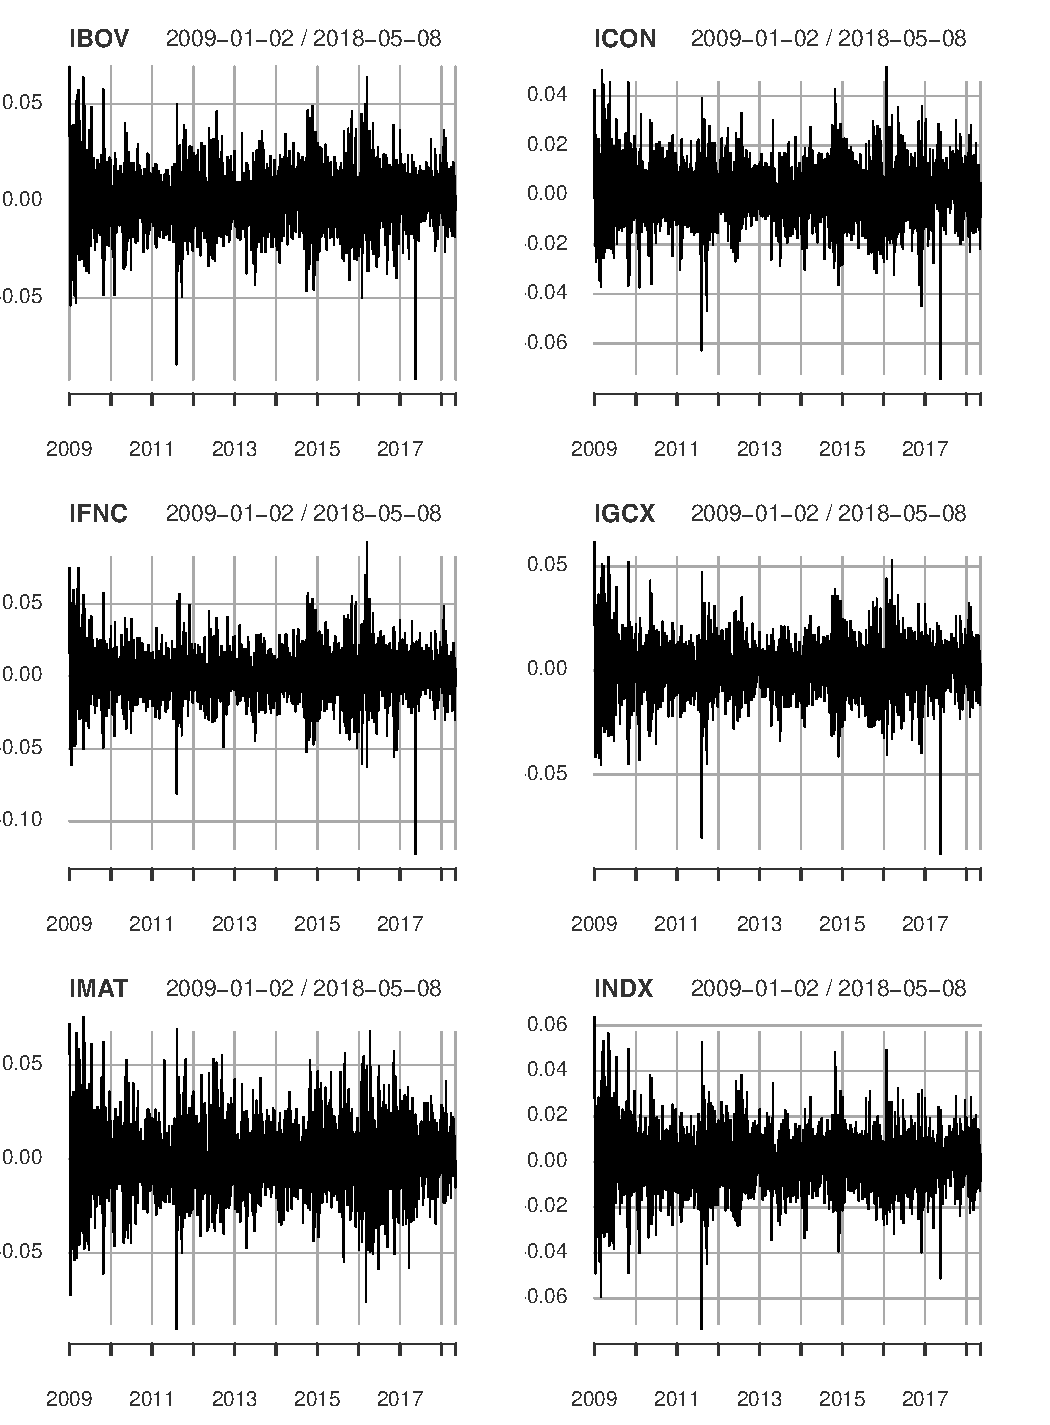
\includegraphics[width=1\linewidth]{figs/artigo-retornos}
	\caption{Retornos dos índices do estudo. Período completo entre 02/01/2009 a 08/05/2018.}
	\label{fig:artigo-retornos}
\end{figure}

\begin{figure}[H]
	\centering
	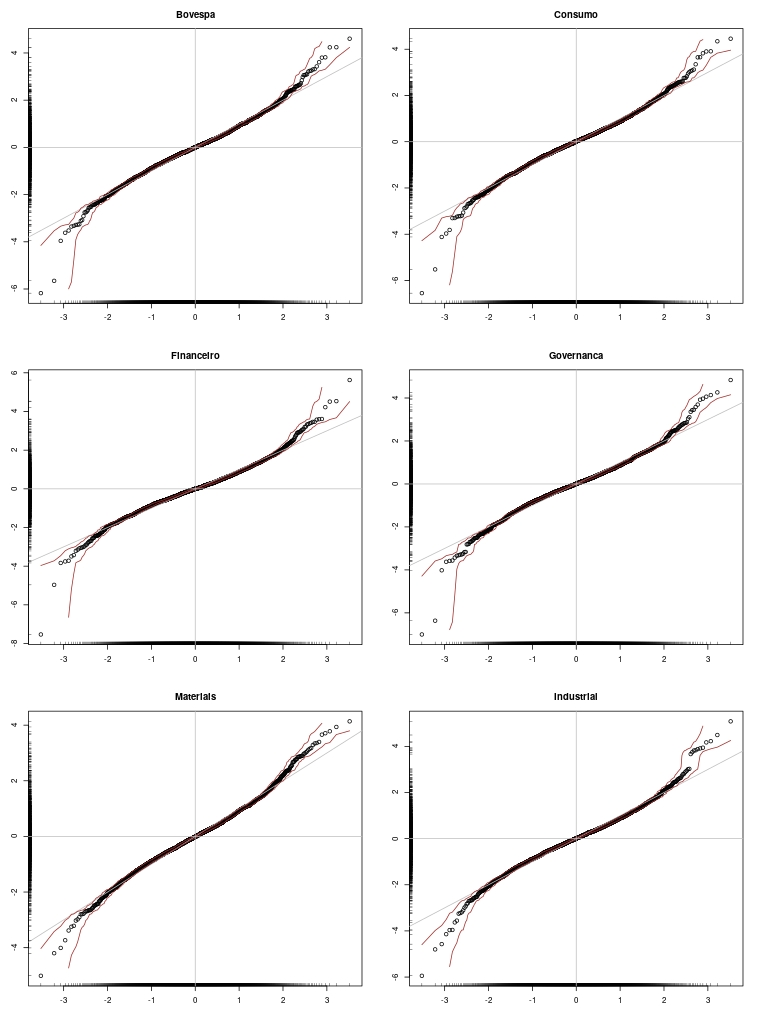
\includegraphics[width=1\linewidth]{figs/artigo-qqplots}
	\caption{Análise de normalidade dos retornos através de gráficos quantil-quantil.}
	\label{fig:artigo-qqplots}
\end{figure}


%% Figuras com os gráficos ACF antes e depois da filtragem eGARCH
%\begin{figure}[H]
%	\centering
%	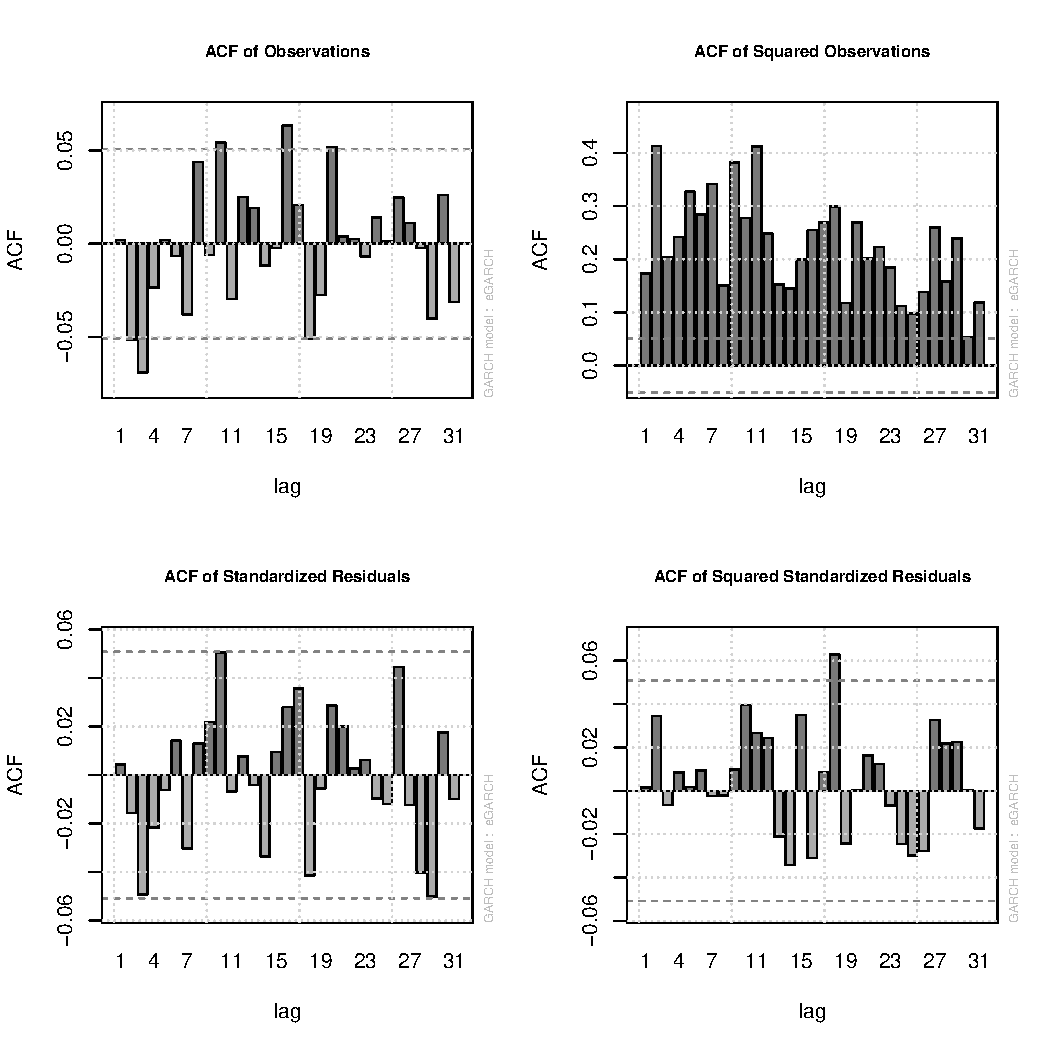
\includegraphics[width=1\linewidth]{figs/artigo-acf-IBovespa}
%	\caption{Ibovespa. Na parte superior está o ACF das perdas observadas e seus quadrados, enquanto que na parte inferior os resíduos padronizados e seus quadrados após a modelagem eGARCH. Período dentro da amostra 01/01/2013 a 31/12/2008.}
%	\label{fig:artigo-acf-ibovespa}
%\end{figure}
%
%\begin{figure}[H]
%	\centering
%	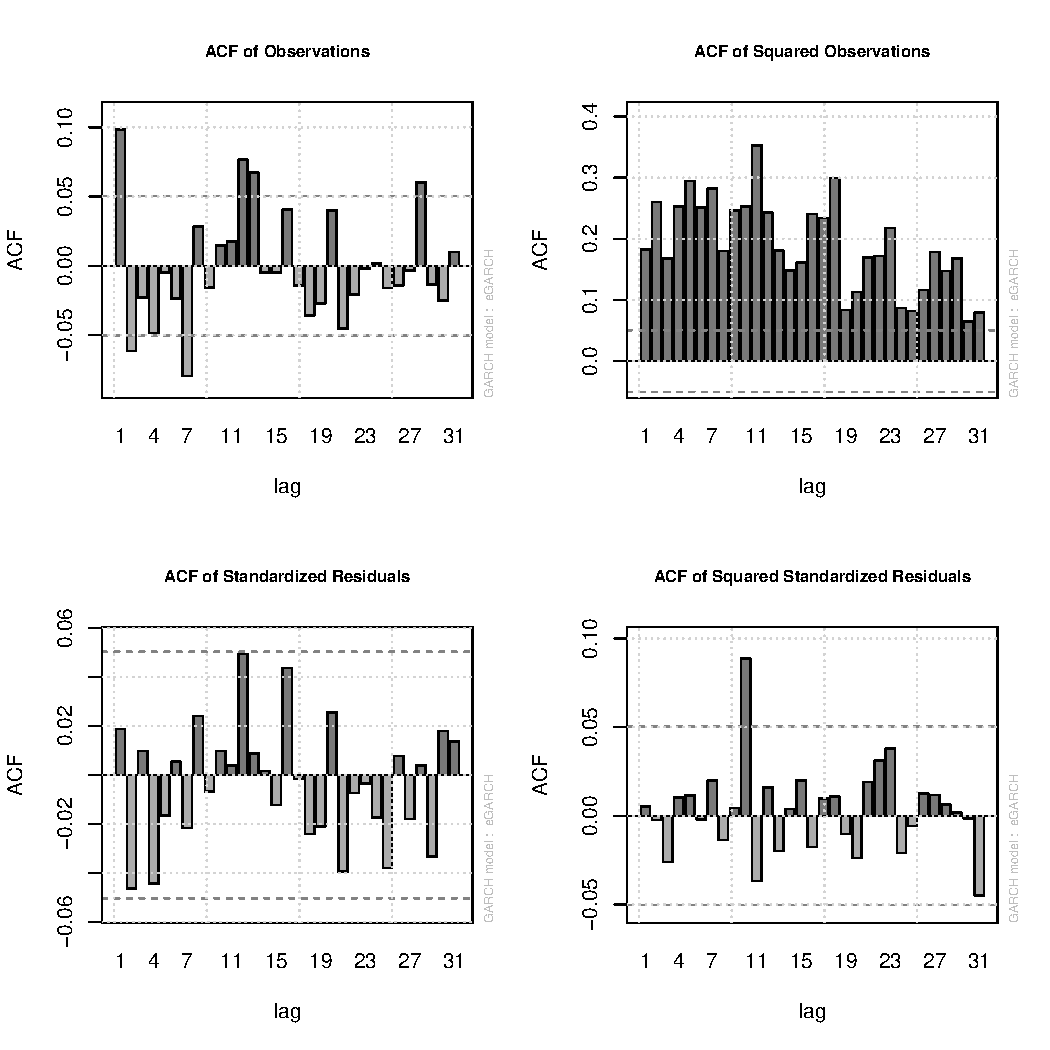
\includegraphics[width=1\linewidth]{figs/artigo-acf-IPC}
%	\caption{IPC. Na parte superior está o ACF das perdas observadas e seus quadrados, enquanto que na parte inferior os resíduos padronizados e seus quadrados após a modelagem eGARCH. Período dentro da amostra 01/01/2013 a 31/12/2008.}
%	\label{fig:artigo-acf-ipc}
%\end{figure}
%
%\begin{figure}[H]
%	\centering
%	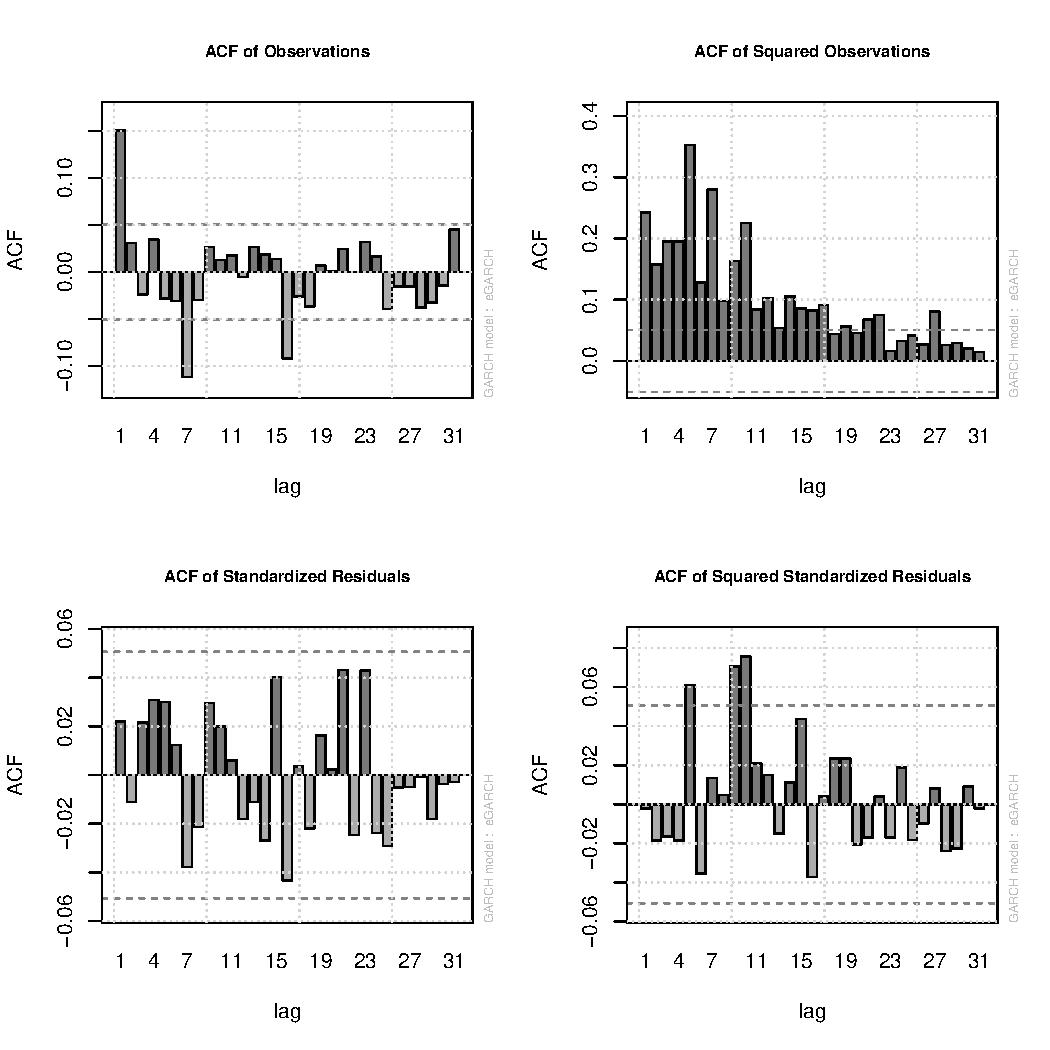
\includegraphics[width=1\linewidth]{figs/artigo-acf-IPSA}
%	\caption{IPSA. Na parte superior está o ACF das perdas observadas e seus quadrados, enquanto que na parte inferior os resíduos padronizados e seus quadrados após a modelagem eGARCH. Período dentro da amostra 01/01/2013 a 31/12/2008.}
%	\label{fig:artigo-acf-ipsa}
%\end{figure}
%
%\begin{figure}[H]
%	\centering
%	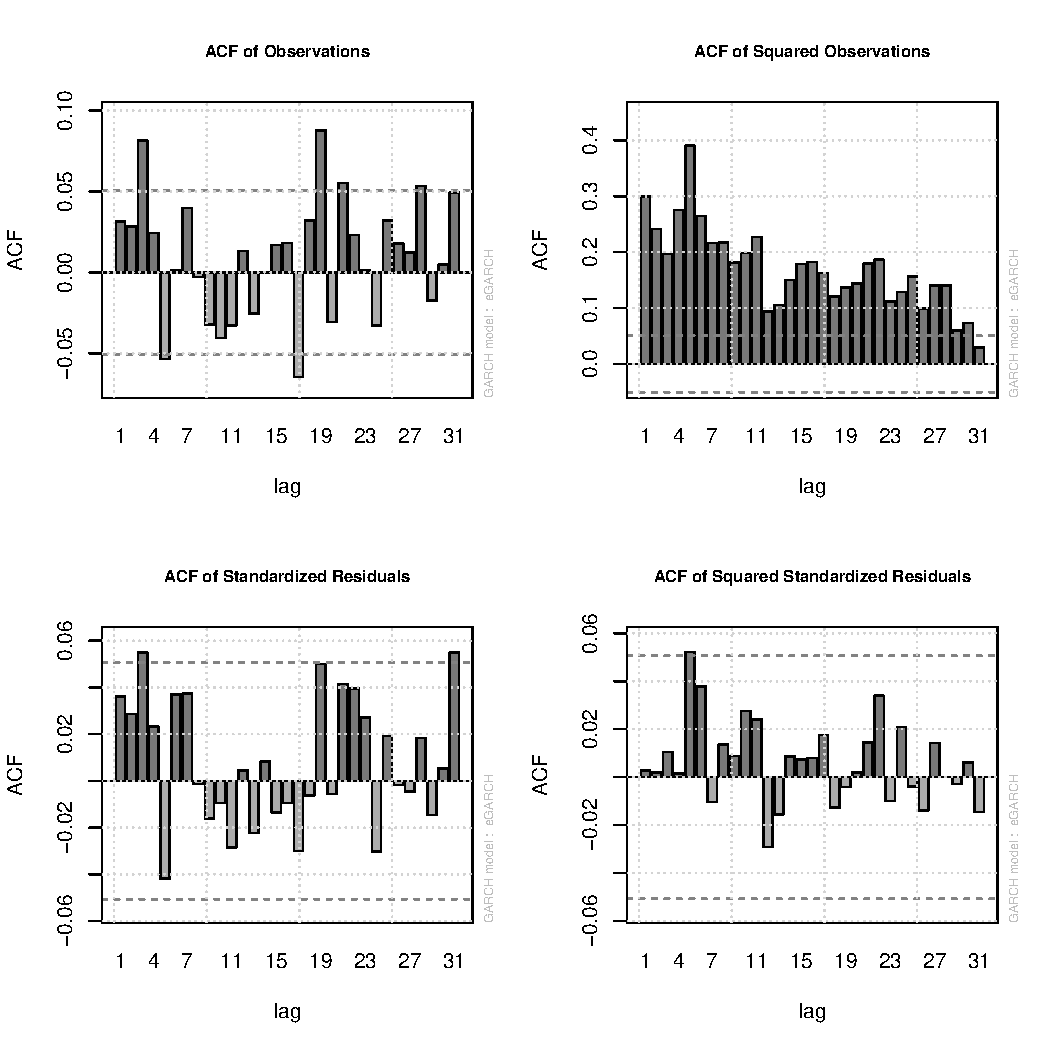
\includegraphics[width=1\linewidth]{figs/artigo-acf-Merval}
%	\caption{Merval. Na parte superior está o ACF das perdas observadas e seus quadrados, enquanto que na parte inferior os resíduos padronizados e seus quadrados após a modelagem eGARCH. Período dentro da amostra 01/01/2013 a 31/12/2008.}
%	\label{fig:artigo-acf-merval}
%\end{figure}
%
%\begin{figure}[H]
%	\centering
%	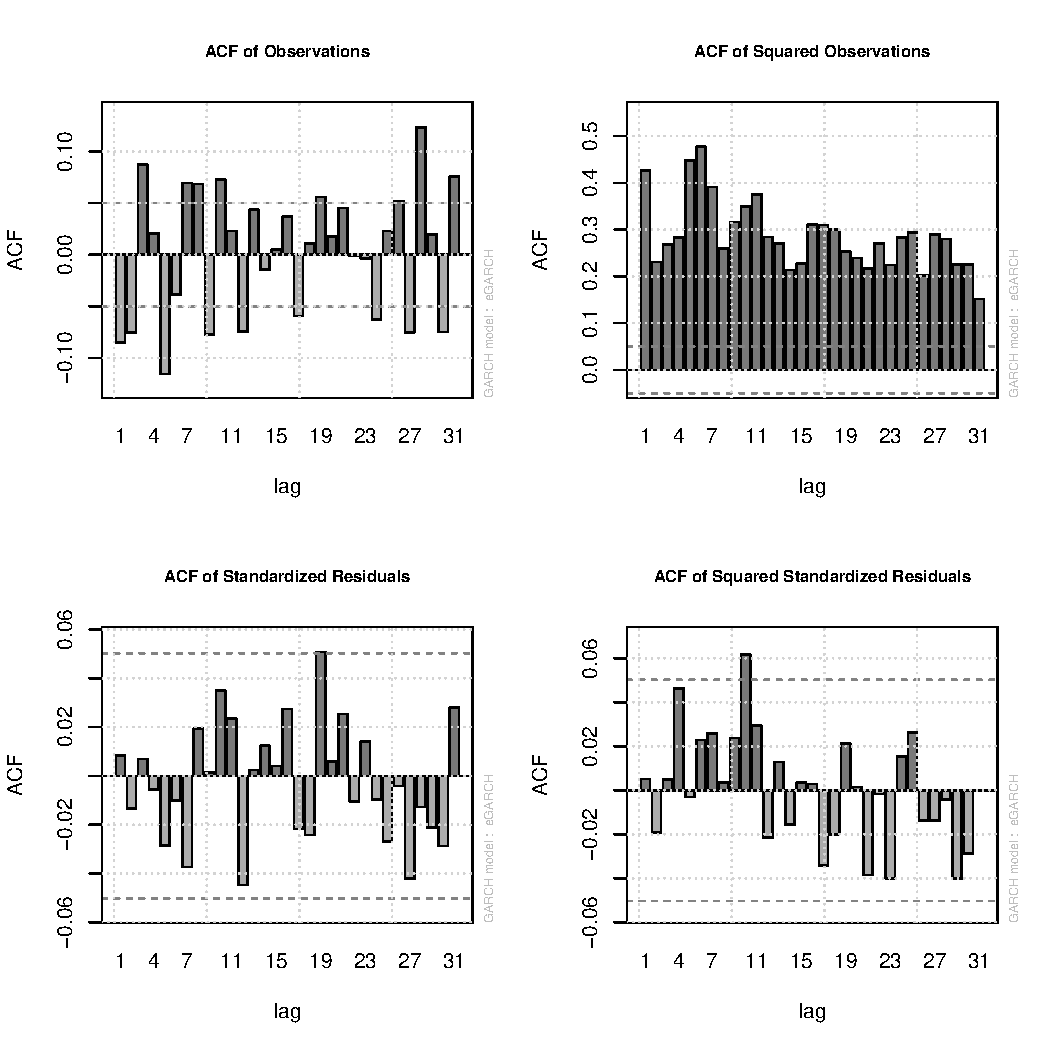
\includegraphics[width=1\linewidth]{figs/artigo-acf-SP-TSE}
%	\caption{S\&P TSE. Na parte superior está o ACF das perdas observadas e seus quadrados, enquanto que na parte inferior os resíduos padronizados e seus quadrados após a modelagem eGARCH. Período dentro da amostra 01/01/2013 a 31/12/2008.}
%	\label{fig:artigo-acf-sptse}
%\end{figure}
%
%\begin{figure}[H]
%	\centering
%	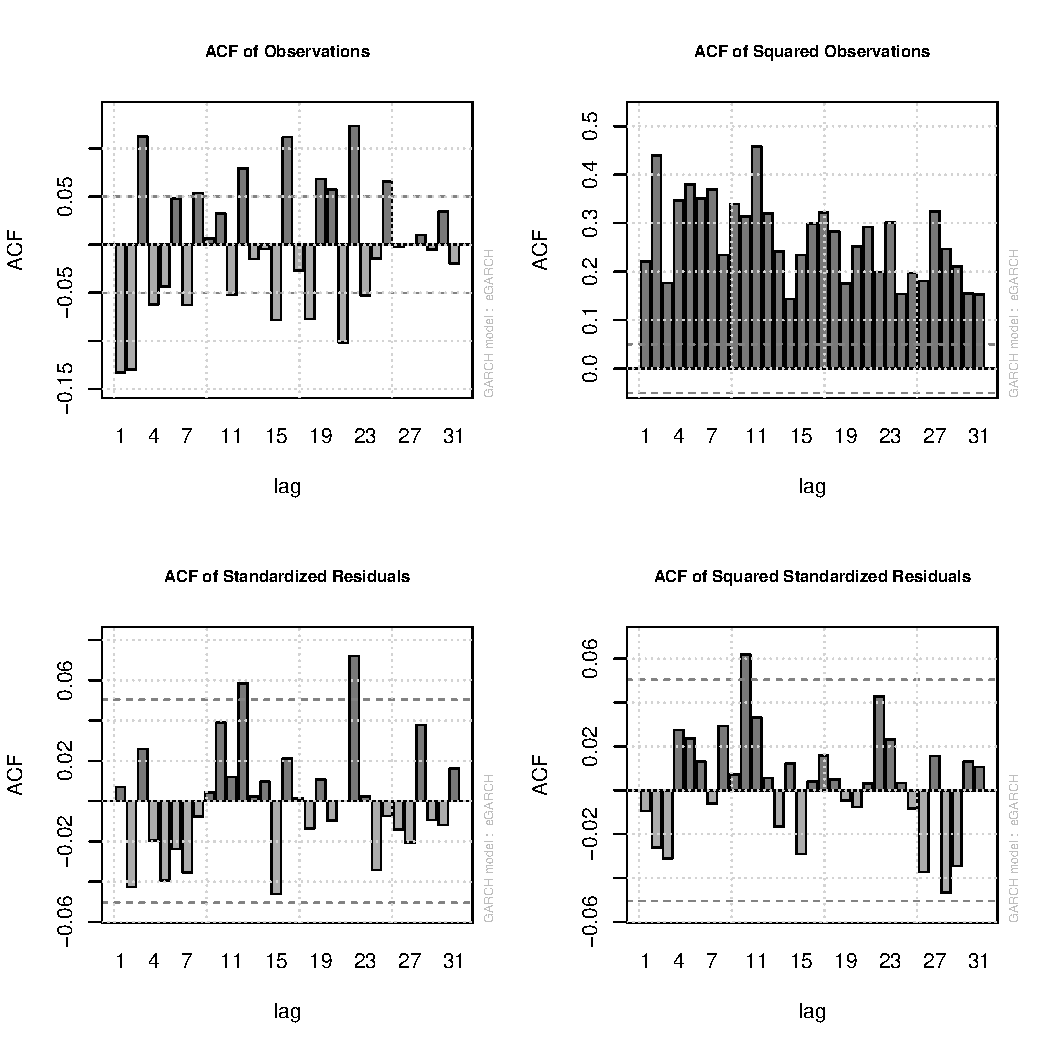
\includegraphics[width=1\linewidth]{figs/artigo-acf-SP500}
%	\caption{S\&P500. Na parte superior está o ACF das perdas observadas e seus quadrados, enquanto que na parte inferior os resíduos padronizados e seus quadrados após a modelagem eGARCH. Período dentro da amostra 01/01/2013 a 31/12/2008.}
%	\label{fig:artigo-acf-sp500}
%\end{figure}

\begin{figure}[H]
	\centering
	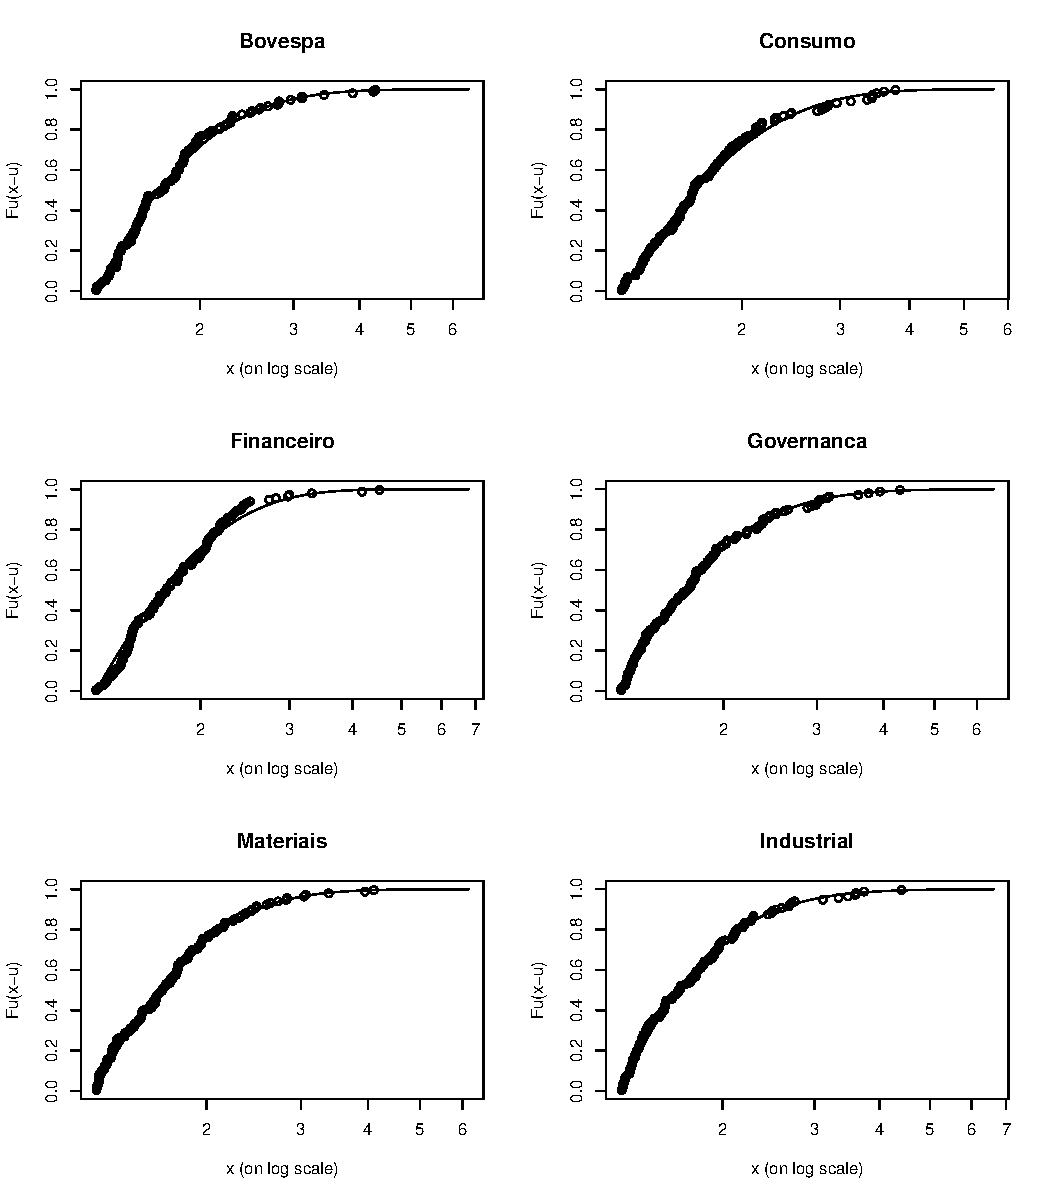
\includegraphics[width=1\linewidth]{figs/artigo-gpdfit}
	\caption{Qualidade do ajuste dos dados de inovações em excesso contra uma GPD de referência. Período dentro da amostra.}
	\label{fig:artigo-gpdfit}
\end{figure}

\begin{figure}[H]
	\centering
	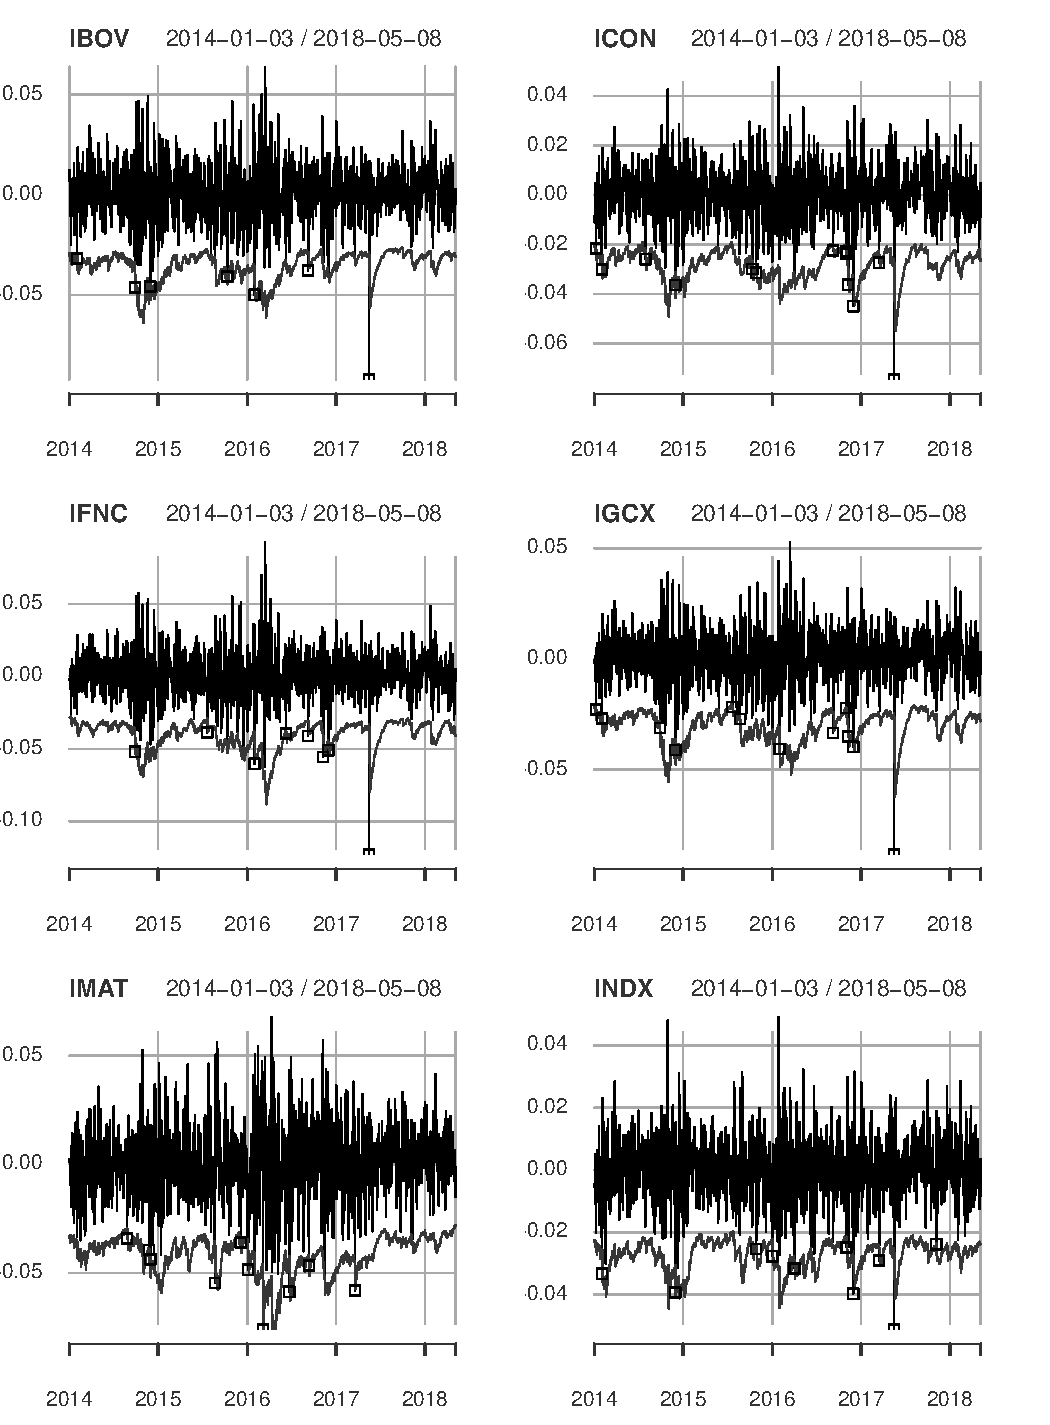
\includegraphics[width=1\linewidth]{figs/artigo-backtest}
	\caption{$VaR_{99\%}$ no modelo EVT condicional para todos os índices. Violações demarcadas.}
	\label{fig:artigo-backtest}
\end{figure}

\begin{figure}[H]
	\centering
	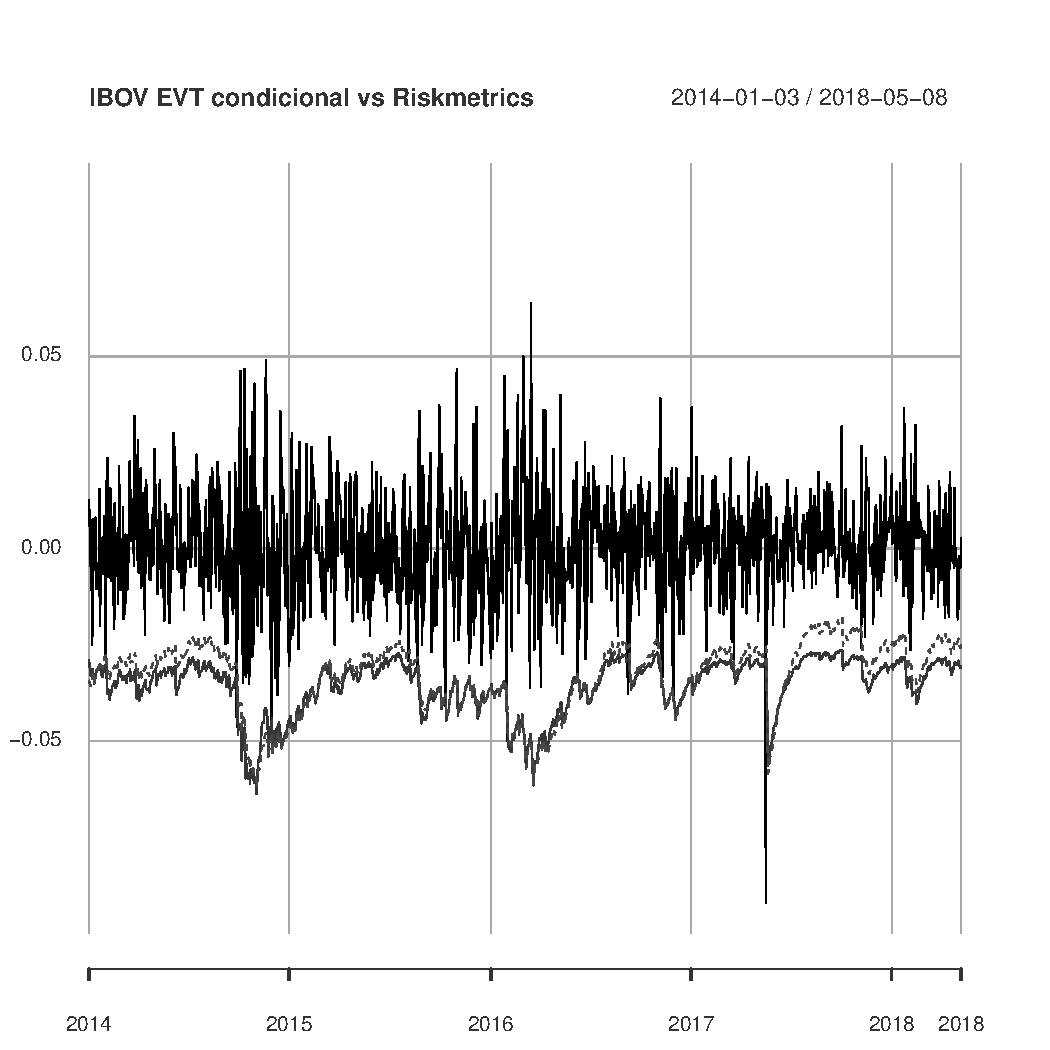
\includegraphics[width=1\linewidth]{figs/artigo-ibovevt}
	\caption{Teste fora da amostra para o IBOV. O modelo EVT condicional (linha sólida) possui menor taxa de decaimento após um choque de volatilidde que o modelo Riskmetrics (linha tracejada).}
	\label{fig:artigo-ibovevt}
\end{figure}

\end{document}
